% !TEX TS-program = pdflatex
% !TEX root = Tes.tex
% !TEX spellcheck = en-EN

\documentclass[12pt,%                      % corpo del font principale
               a4paper,%                   % A4 papers
               %twoside,openright,%         % twoside with free right side
               oneside,openany,%           % one side
               titlepage,%                 % use a titlepage
               headinclude,footinclude,%  % header and foot header
               BCOR5mm,%                   % rilegatura di 5 mm
               cleardoublepage=empty,%     % empty pages with no header and foot
               tablecaptionabove,%         % table caption above tables
               floatperchapter,
               ]{scrreprt}                 % KOMA-Script report class;


\usepackage{braket}
\usepackage{changepage}
\usepackage[english]{babel}	% latest language is predefined
\usepackage[T1]{fontenc}		% font coding


\usepackage{indentfirst}		% indent first paragraph of each section
\usepackage{mparhack,fixltx2e,relsize}	% fancy typographies stuff

\usepackage[eulerchapternumbers,%	% chapter font Euler
            subfig,%			% in subfig objects
            beramono,%			% Bera Mono as fixed spacing font
            eulermath,%			% AMS Euler as math font
            pdfspacing,%		% improves line filling
            listings,%			% code output
 %          parts,%			% uncomment for a document divided in parts
            listsseparated,
            ]{classicthesis}		% style ClassicThesis
%\setlength{\cftbeforeloftitleskip}{100pt}
%\renewcommand{\cftbeforeloftitleskip}{1000pt}

\usepackage{arsclassica}		% modifies some aspects of ClassicThesis package
\let\marginpar\oldmarginpar		% for margin notes with \todonotes (overwise conflict with the new definition of \marginpar in classic thesis)
\usepackage[shadow]{todonotes}			% for margin notes and comments

\usepackage{bookmark}			% bookmarks

%*********************************************************************************
% Bibliography
%*********************************************************************************
%%\usepackage[style=authoryear,hyperref,backref,natbib, ,maxcitenames=1, mincitenames = 1, citestyle=authoryear-comp, backend=biber,sortcites,sorting=ynt]{biblatex}
%\usepackage[style=numeric,hyperref,backref,natbib]{biblatex}




%*********************************************************************************
% Graphics
%*********************************************************************************
\usepackage{graphicx}			% images
\usepackage{subfigure}
\usepackage{wrapfig}
\usepackage{tikz}
\usetikzlibrary{mindmap,trees}
\usetikzlibrary{backgrounds}
\usepackage{verbatim}
\usepackage[dvipsnames]{xcolor}
% \usepackage{morefloats}
%\usepackage{chngcntr}
\usepackage{pdfpages}
\usepackage{braket}
\usepackage{amssymb}
\def\delequal{\mathrel{\ensurestackMath{\stackon[1pt]{=}{\scriptstyle\Delta}}}}
\usepackage{lscape}


%*********************************************************************************
% Tables
%*********************************************************************************
\usepackage{tabularx}			% table of predefined length
\usepackage{siunitx}
\usepackage{pbox}
\usepackage{colortbl}
\usepackage{multirow}
\usepackage{booktabs}
\usepackage{rotating}
\usepackage{hhline}
\setlength\tabcolsep{3pt}
\usepackage{changepage}
% \usepackage[showframe=true]{geometry}

%*********************************************************************************
% Mathematics and symbols
%*********************************************************************************
\usepackage{amsmath, amssymb, amsthm}	% mathematics stuff
\usepackage{mathrsfs}
\usepackage{calc}
\usepackage{algorithmic}
\usepackage[ruled]{algorithm}
\usepackage{latexsym}
\usepackage[geometry]{ifsym}
\usepackage{mathabx}
\usepackage{pifont}

%*********************************************************************************
% Personal
%*********************************************************************************
\usepackage[font=itshape]{quoting}			% fancy quotation packages. [font=small] old option
\usepackage[english]{varioref}		% complete reference package
\usepackage{hyperref}
\usepackage{url}
\usepackage[intoc, english, noprefix]{nomencl}	%for list of symbols
\usepackage[normalem]{ulem}
\usepackage{chemfig} %for chemical formulas
\usepackage{eurosym}			% euro symbol
\usepackage{epigraph}
\usepackage{calligra}
\usepackage{soul}
\usepackage[utf8]{inputenc}

\definecolor{codegreen}{rgb}{0,0.6,0}
\definecolor{codegray}{rgb}{0.5,0.5,0.5}
\definecolor{codepurple}{rgb}{0.58,0,0.82}
\definecolor{backcolour}{rgb}{0.95,0.95,0.92}


\setlength{\epigraphwidth}{\textwidth}



%*********************************************************************************
% Calling personal settings and making nomenclature
%*********************************************************************************
%*********************************************************************************
% Personal commands
%*********************************************************************************
\newcommand{\myName}{Marzio De Corato }	% author
\newcommand{\myTitle}{Hazardous asteroids forecast via Markov random fields - Project for the course Probabilistic modelling (DSE)}	% title
\newcommand{\myDegree}{Data Science and Economics}	% thesis type
\newcommand{\myUni}{Unimi}	% institute
\newcommand{\myLocation}{Milan}	% place
\newcommand{\myTime}{\today}	% date

%*************************
%Scaling tikz mindmaps
%******************
\makeatletter
\def\hlinewd#1{%
\noalign{\ifnum0=`}\fi\hrule \@height #1 %
\futurelet\reserved@a\@xhline}
\makeatother

%*********************************************************************************
% General math defs
%*********************************************************************************
\newcommand{\beq}{\begin{equation}}
\newcommand{\eeq}{\end{equation}}

\newcommand{\bea}{\begin{eqnarray}}
\newcommand{\eea}{\end{eqnarray}}

\setdoublesep{.5ex}
\renewcommand*\printatom[1]{\ensuremath{\mathsf{#1}}}
\setatomsep{2em}

\newcommand{\barray}{\begin{equation}\begin{array}}
\newcommand{\earray}{\end{array}\end{equation}}


%*********************************************************************************
% General shortcuts
%*********************************************************************************

\newcommand{\bit}{\begin{itemize}}
\newcommand{\eit}{\end{itemize}}

\newcommand{\bfig}{\begin{figure}}
\newcommand{\efig}{\end{figure}}

\newcommand{\btable}{\begin{table}}
\newcommand{\etable}{\end{table}}

\newcommand{\btabular}{\begin{tabular}}
\newcommand{\etabular}{\end{tabular}}

\newcommand{\benum}{\begin{enumerate}}
\newcommand{\eenum}{\end{enumerate}}


\newcommand{\red}{\textcolor{red}}

%*********************************************************************************
% Nomenclature
%*********************************************************************************

\newcommand{\ucSiC}{$\mu$c-Si$_{1-x}$C$_x$}
\newcommand{\aSiC}{a-Si$_{1-x}$C$_x$}
\newcommand{\ucSi}{$\mu$c-Si}
\newcommand{\SW}{Staebler-Wronski}
\newcommand{\methane}{CH$_4$}
\newcommand{\silane}{SiH$_4$}
\newcommand{\hydrogen}{H$_2$}
\newcommand{\SiF}{SiF$_{4}$}

\newcommand{\fRaman}{f_c^{\text{\footnotesize Raman}}}
\newcommand{\fhexagXRD}{f_{\text{hex}}^{\text{\scriptsize XRD}}}
\newcommand{\fhexagRaman}{f_{\text{hex}}^{\text{\scriptsize Raman}}}
\newcommand{\WRF}{$W_{\text{RF}}$}
\newcommand{\wRF}{$w_{\text{RF}}$}
\newcommand{\SigmaDark}{$\sigma_{\text{dark}}$}
\newcommand{\SigmaPh}{$\sigma_{\text{ph}}$}
\newcommand{\Eg}{$E_g$}
\newcommand{\Eo}{$E_{04}$}
\newcommand{\Ea}{$E_a$}
\newcommand{\Ld}{$L_d$}
\newcommand{\AD}{{\bf AD}}
\newcommand{\LS}{{\bf LS}}
\newcommand{\Ann}{{\bf A}}
\newcommand{\seedLayer}{\emph{``seed layer''}}
\newcommand{\Ram}{$R_{amorph}$}
\newcommand{\Jo}{$J_0$}
\newcommand{\Voc}{$V_{oc}$}
\newcommand{\Jsc}{$J_{sc}$}
\newcommand{\JV}{$J(V)$}
\newcommand{\FF}{$FF$}
\newcommand{\R}{$R_C$}
\newcommand{\ucSiO}{$\mu$c-SiO$_x$}
\newcommand{\SETCHa}{SET$_{CH_4 1}$}
\newcommand{\SETCHb}{SET$_{CH_4 2}$}
\newcommand{\SETCHc}{SET$_{CH_4 3}$}
\newcommand{\SETWRFa}{SET$_{w_{RF} 1}$}
\newcommand{\SETWRFb}{SET$_{w_{RF} 2}$}
\newcommand{\SETSiFa}{SET$_{SiF_4 1}$}
\newcommand{\SETSiFb}{SET$_{SiF_4 2}$}
\newcommand{\SETSiFc}{SET$_{SiF_4 3}$}
\newcommand{\SETp}{SET$_{\text{peaks}}$}
\newcommand{\SETv}{SET$_{\text{valleys}}$}
\newcommand{\SETTa}{SET$_{T 1}$}
\newcommand{\SETTb}{SET$_{T 2}$}
\newcommand{\Vcoll}{$V_{coll}$}

%*********************************************************************************
% Units
%*********************************************************************************

\newcommand{\cm}{cm$^{-1}$}
\newcommand{\mWcm}{mW/cm$^2$}

%*********************************************************************************
% Symbols
%*********************************************************************************
\newcommand{\FC}{\FilledCircle}
\newcommand{\FTU}{\FilledTriangleUp}
\newcommand{\FTL}{\FilledTriangleLeft}
\newcommand{\FTR}{\FilledTriangleRight}
\newcommand{\FD}{\FilledDiamondshape}
\newcommand{\FS}{\FilledSquare}
\newcommand{\Fstar}{$\bigstar$}
      



% Commands for ensembles (serve il pacchetto amssymb)
\newcommand{\numberset}{\mathbb} 
\newcommand{\N}{\numberset{N}} 

% environment for systems
\newenvironment{sistema}%
  {\left\lbrace\begin{array}{@{}l@{}}}%
  {\end{array}\right.}

% definitions (requires amsthm)
\theoremstyle{definition} 
\newtheorem{definizione}{Definizione}

% teoremi, leggi e decreti (serve il pacchetto amsthm)
\theoremstyle{plain} 
\newtheorem{theorem}{Theorem}
\newtheorem{law}{Law}
%\newtheorem{decreto}[legge]{Decreto}
%\newtheorem{murphy}{Murphy}[section]


%*********************************************************************************
% Settings chapter title
%*********************************************************************************
\titleformat{\chapter}[hang]% "hang" instead of "block"
    {\normalfont\Large\sffamily}%
    {{\color{halfgray}\chapterNumber\thechapter%
    \hspace{10pt}\vline}  }{10pt}%
    {\spacedallcaps}

\newenvironment{unnumbered}%
{\setcounter{secnumdepth}{-1}}
{\setcounter{secnumdepth}{2}}

%*********************************************************************************
% Settings biblatex
%*********************************************************************************
%\defbibheading{bibliography}{%
%\cleardoublepage
%\manualmark
%\phantomsection 
%\addcontentsline{toc}{chapter}{\tocEntry{\bibname}}
%\chapter*{\bibname\markboth{\spacedlowsmallcaps{\bibname}}
%{\spacedlowsmallcaps{\bibname}}}}



%*********************************************************************************
% Settings listings
%*********************************************************************************
\lstset{language=[LaTeX]Tex,%C++,
    keywordstyle=\color{RoyalBlue},%\bfseries,
    basicstyle=\small\ttfamily,
    %identifierstyle=\color{NavyBlue},
    commentstyle=\color{Green}\ttfamily,
    stringstyle=\rmfamily,
    numbers=none,%left,%
    numberstyle=\scriptsize,%\tiny
    stepnumber=5,
    numbersep=8pt,
    showstringspaces=false,
    breaklines=true,
    frameround=ftff,
    frame=single
} 



%*********************************************************************************
% Settings hyperref
%*********************************************************************************
\hypersetup{%
    hyperfootnotes=false,pdfpagelabels,
    %draft,	% = elimina tutti i link (utile per stampe in bianco e nero)
    colorlinks=true, linktocpage=true, pdfstartpage=1, pdfstartview=FitV,%
    % decommenta la riga seguente per avere link in nero (per esempio per la stampa in bianco e nero)
    %colorlinks=false, linktocpage=false, pdfborder={0 0 0}, pdfstartpage=1, pdfstartview=FitV,% 
    breaklinks=true, pdfpagemode=UseNone, pageanchor=true, pdfpagemode=UseOutlines,%
    plainpages=false, bookmarksnumbered, bookmarksopen=true, bookmarksopenlevel=1,%
    hypertexnames=true, pdfhighlight=/O,%nesting=true,%frenchlinks,%
    urlcolor=webbrown, linkcolor=RoyalBlue, citecolor=webgreen, %pagecolor=RoyalBlue,%
    %urlcolor=Black, linkcolor=Black, citecolor=Black, %pagecolor=Black,%
    pdftitle={\myTitle},%
    pdfauthor={\textcopyright\ \myName, \myUni, \myFaculty},%
    pdfsubject={},%
    pdfkeywords={},%
    pdfcreator={pdfLaTeX},%
    pdfproducer={LaTeX with hyperref and ClassicThesis}%
}

%*********************************************************************************
% Margins settings optimized for  A4 format
%*********************************************************************************
\areaset[current]{336pt}{750pt}
\setlength{\marginparwidth}{7em}
\setlength{\marginparsep}{2em}%




%\hyphenation{Fortran ma-cro-istru-zio-ne nitro-idrossil-amminico}
\hyphenation{anisotropies an-i-so-trop-ies}
  % general custom settings (margins etc)

% \makenomenclature
% \renewcommand{\nomname}{List of Symbols and Abbreviations}

\bibliographystyle{plain}

\begin{document}



%----------------------------------------------------------------------------------------
%	TITLE AND AUTHOR(S)
%----------------------------------------------------------------------------------------

\title{\normalfont\spacedallcaps{Hazardous asteroids forecast via Markov random fields}} % The article title

\subtitle{Project for the course Probabilistic modelling (DSE)} % Uncomment to display a subtitle

\author{
  Marzio De Corato
}

\date{} % An optional date to appear under the author(s)

%----------------------------------------------------------------------------------------


%----------------------------------------------------------------------------------------
%	TABLE OF CONTENTS & LISTS OF FIGURES AND TABLES
%----------------------------------------------------------------------------------------

\maketitle % Print the title/author/date block

%\setcounter{tocdepth}{2} % Set the depth of the table of contents to show sections and subsections only



%\listoffigures % Print the list of figures%

%\listoftables % Print the list of tables

\newpage
\begin{figure}[h]
\begin{center}
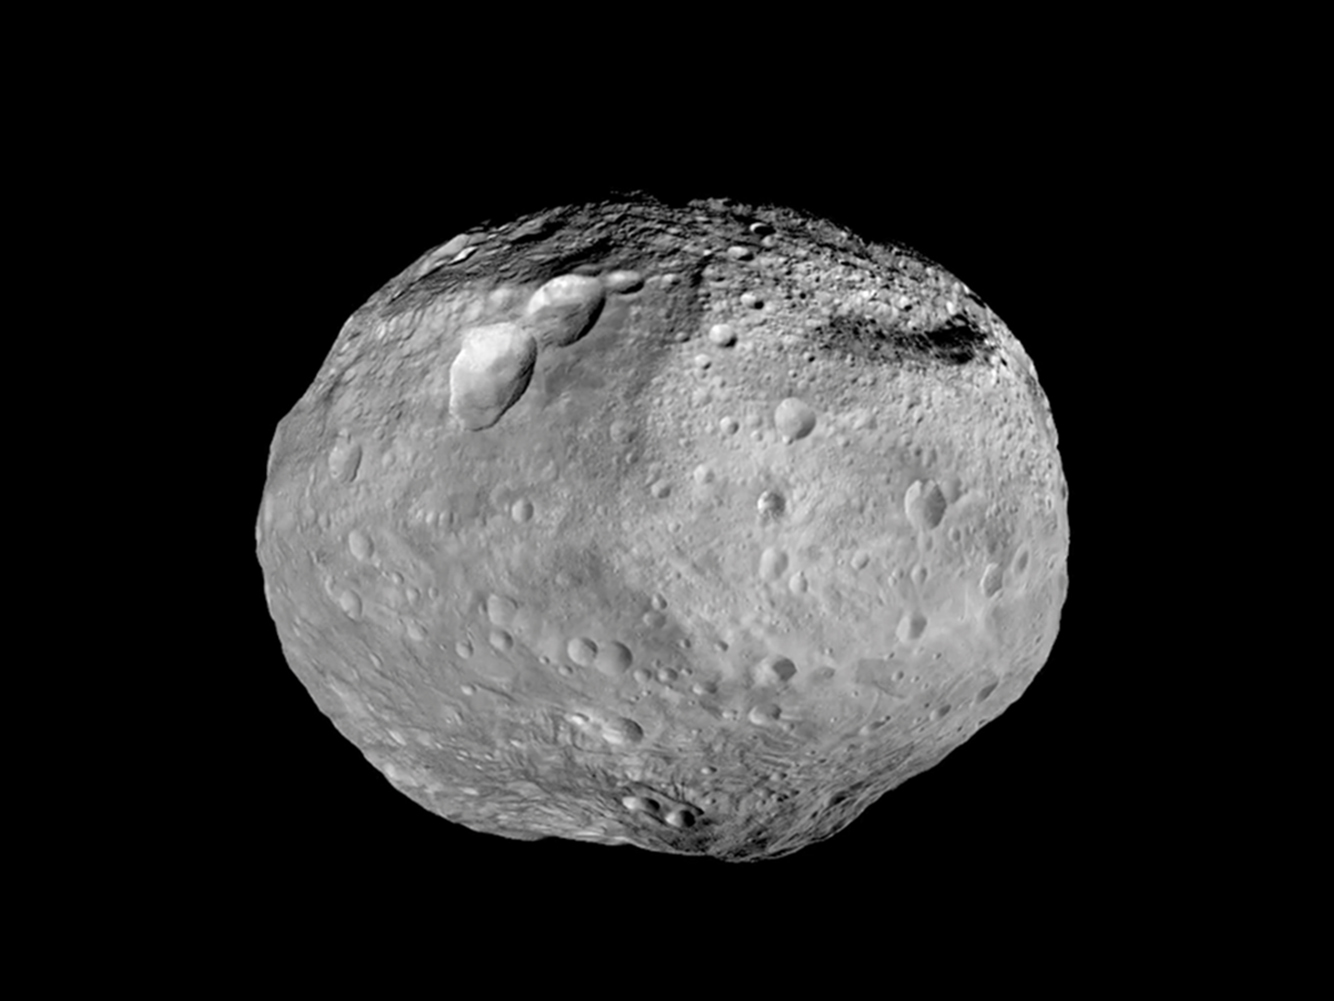
\includegraphics[width=0.6\textwidth]{Figures/vesta_asteroid.jpg}
\captionsetup{labelformat=empty}
\caption{A NASA image of asteroid Vesta as taken by the spacecraft Dawn. Vesta is one of the biggest asteroid in the asteroid belt of solar system (its volume is equal to $7,5\cdot10^{7}$ km$^{3}$. Image taken from \cite{vesta_source}}
\end{center}
\end{figure}
\begin{figure}[h]
\begin{center}
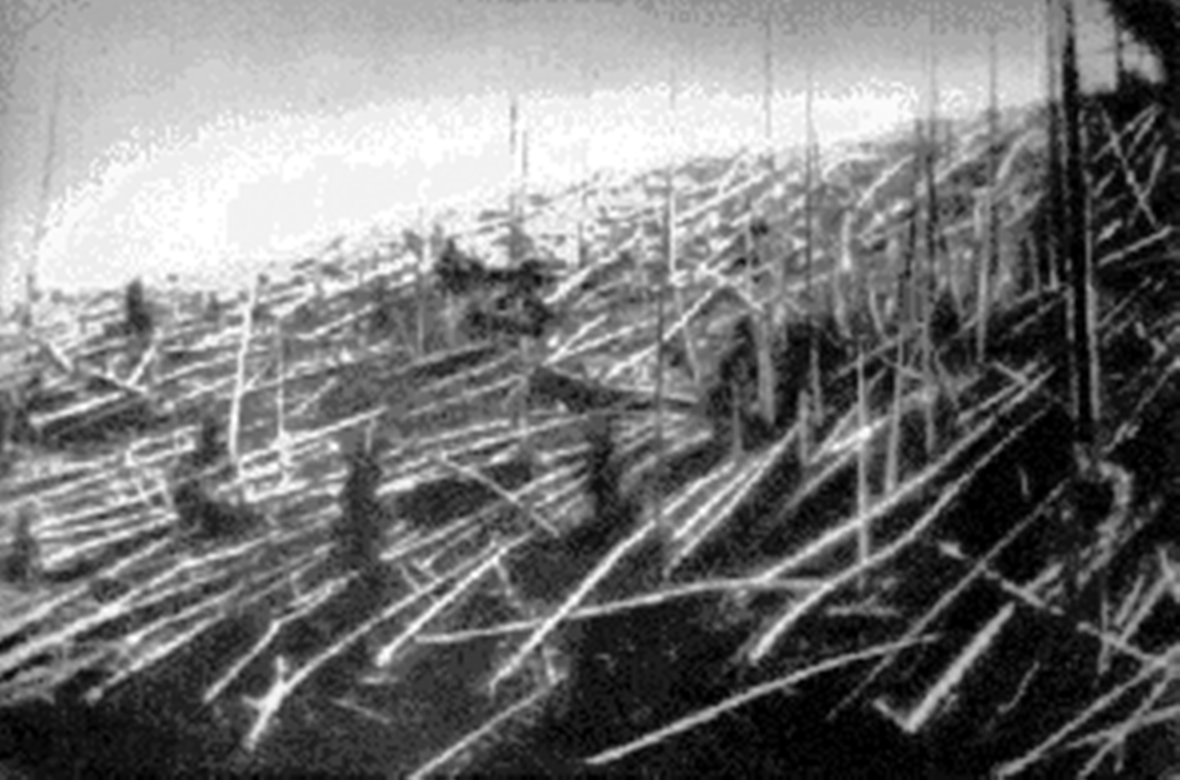
\includegraphics[width=0.6\textwidth]{Figures/Tunguska.png}
\captionsetup{labelformat=empty}
\caption{A picture provided by the Soviet Academy of Science in 1927 of Podkamennaya Tunguska. This place was hit, in 1908, by an asteroid of 50-60 m. Such asteroid flattened almost 80 million trees over an area of 2,150 km$^{2}$. The explosion intensity was near to 12 megatons: for reference the modern US nuclear bomb are in the range of 0.3 kilotons to 1.2 megatons. The Hiroshima bomb was nearly to 15 kilotons. Image taken from \cite{Tunguska_source}}
\end{center}
\end{figure}
\newpage


\epigraph{
\textit{This day may possibly be my last: but the laws of probability, so true in general, so fallacious in particular, still allow about fifteen years. }\\Edward Gibbon (1737-1794)
}

\newpage

\section*{\begin{center}
Abstract
\end{center}}




\newpage

\tableofcontents % Print the table of contents

\newpage % Start the article content on the second page, remove this if you have a longer abstract that goes onto the second page



\newpage
%----------------------------------------------------------------------------------------
%	INTRODUCTION
%----------------------------------------------------------------------------------------

\chapter{Introduction}

The description and the forecast of physical \footnote{Where here physical should be inteded as mesuarable} phenomena can be attacked with two different approaches: starting from a restricted set of principles/axioms one can formulate theoretical models that provide equations that describe such phenomena. Such approach, which will be called here \textit{ab-initio}. On the other side one can start from data and fit them into some general models (with fixed or not fixed number of parameters). This method will be called here as machine learning (ML) method. In the first case one have the advantage to have an almost full explanation of the meaning of the laws obtained and an overall idea of why nature works in this way. The toll that has to be paid in this case is that, since the phenomena are much more complicated with respect to the starting principles, a consistent part of them may be excluded by the assumption made at the beginning. Furthermore the calculation of the solution given the dynamical equation can be computationally expensive\footnote{This is the case for instance of Hartree-Fock method or of Density Functional Theory: such methods rewrite, with some approximations, the Schroedinger equation in to a much more computationally affordable way. However also in this case the solution for solids can be very expensive \cite{martin_2004}} . On the other side, the ML methods since they make much more general assumptions and work directly on data, are not limited to a particular class of phenomena. Therefore they do not require a development of a specific theory as the \textit{ab-initio} one: the same model can be applied to exoplanets habitability as well to credit risk evaluation. The toll that has to be paid in this case it that the underlying mechanism by which a forecast is preferred to another one may be not so interpretable. Such dichotomy between these two methods can be explained with an example taken from astronomy: at the beginning of XX century astronomers know that mercury follows an elliptical orbit that instead of being fixed rotates around the Sun as shown in Fig. \ref{Perihelion_precession2} Such phenomenon is called \textit{Precession of the perihelion of Mercury}. The crucial point is that there was no way to explain from the Newton gravity theory such phenomenon. At this point scholars had two paths: describe its motion with an empirical law (perhaps with an empirical modification of Newtons gravity law) or instead reformulate from scratch the Newton gravity. The second approach was the one followed by A.Einstein with his general relativity theory (further details are given in the A.Zee textbook \cite{zee2013einstein}). The graphical methods represent a good compromise  between these two approaches: they can be used for every physical phenomena and, since they provide the conditional dependencies/independences they also give a fine and intuitive representation  of their mechanisms. Therefore, if the theory of the process is known, one can use this class of algorithm and compare its finding with the theory. In this way one can not only evaluate the quality of the forecasts, but also of the model provided by the graphical methods. The aim of the present work is to perform such analysis for a dataset that contain the features and the hazardousness \footnote{For Earth} of asteroids. For this dataset, indeed, the relationships between the various features are known. The present work is organized as follows: first a brief introduction about the basic theoretical concepts of the statistical methods here used will be provided, then the dataset will be described and finally, the main results here obtained with graphical methods will be presented as compared with other type of machine learning algorithms. Furthermore an appendix about the theoretical concepts of the theory that explains and interconnects the dataset features is also provided at the end of the present work. 


\begin{figure}[h]
\begin{center}
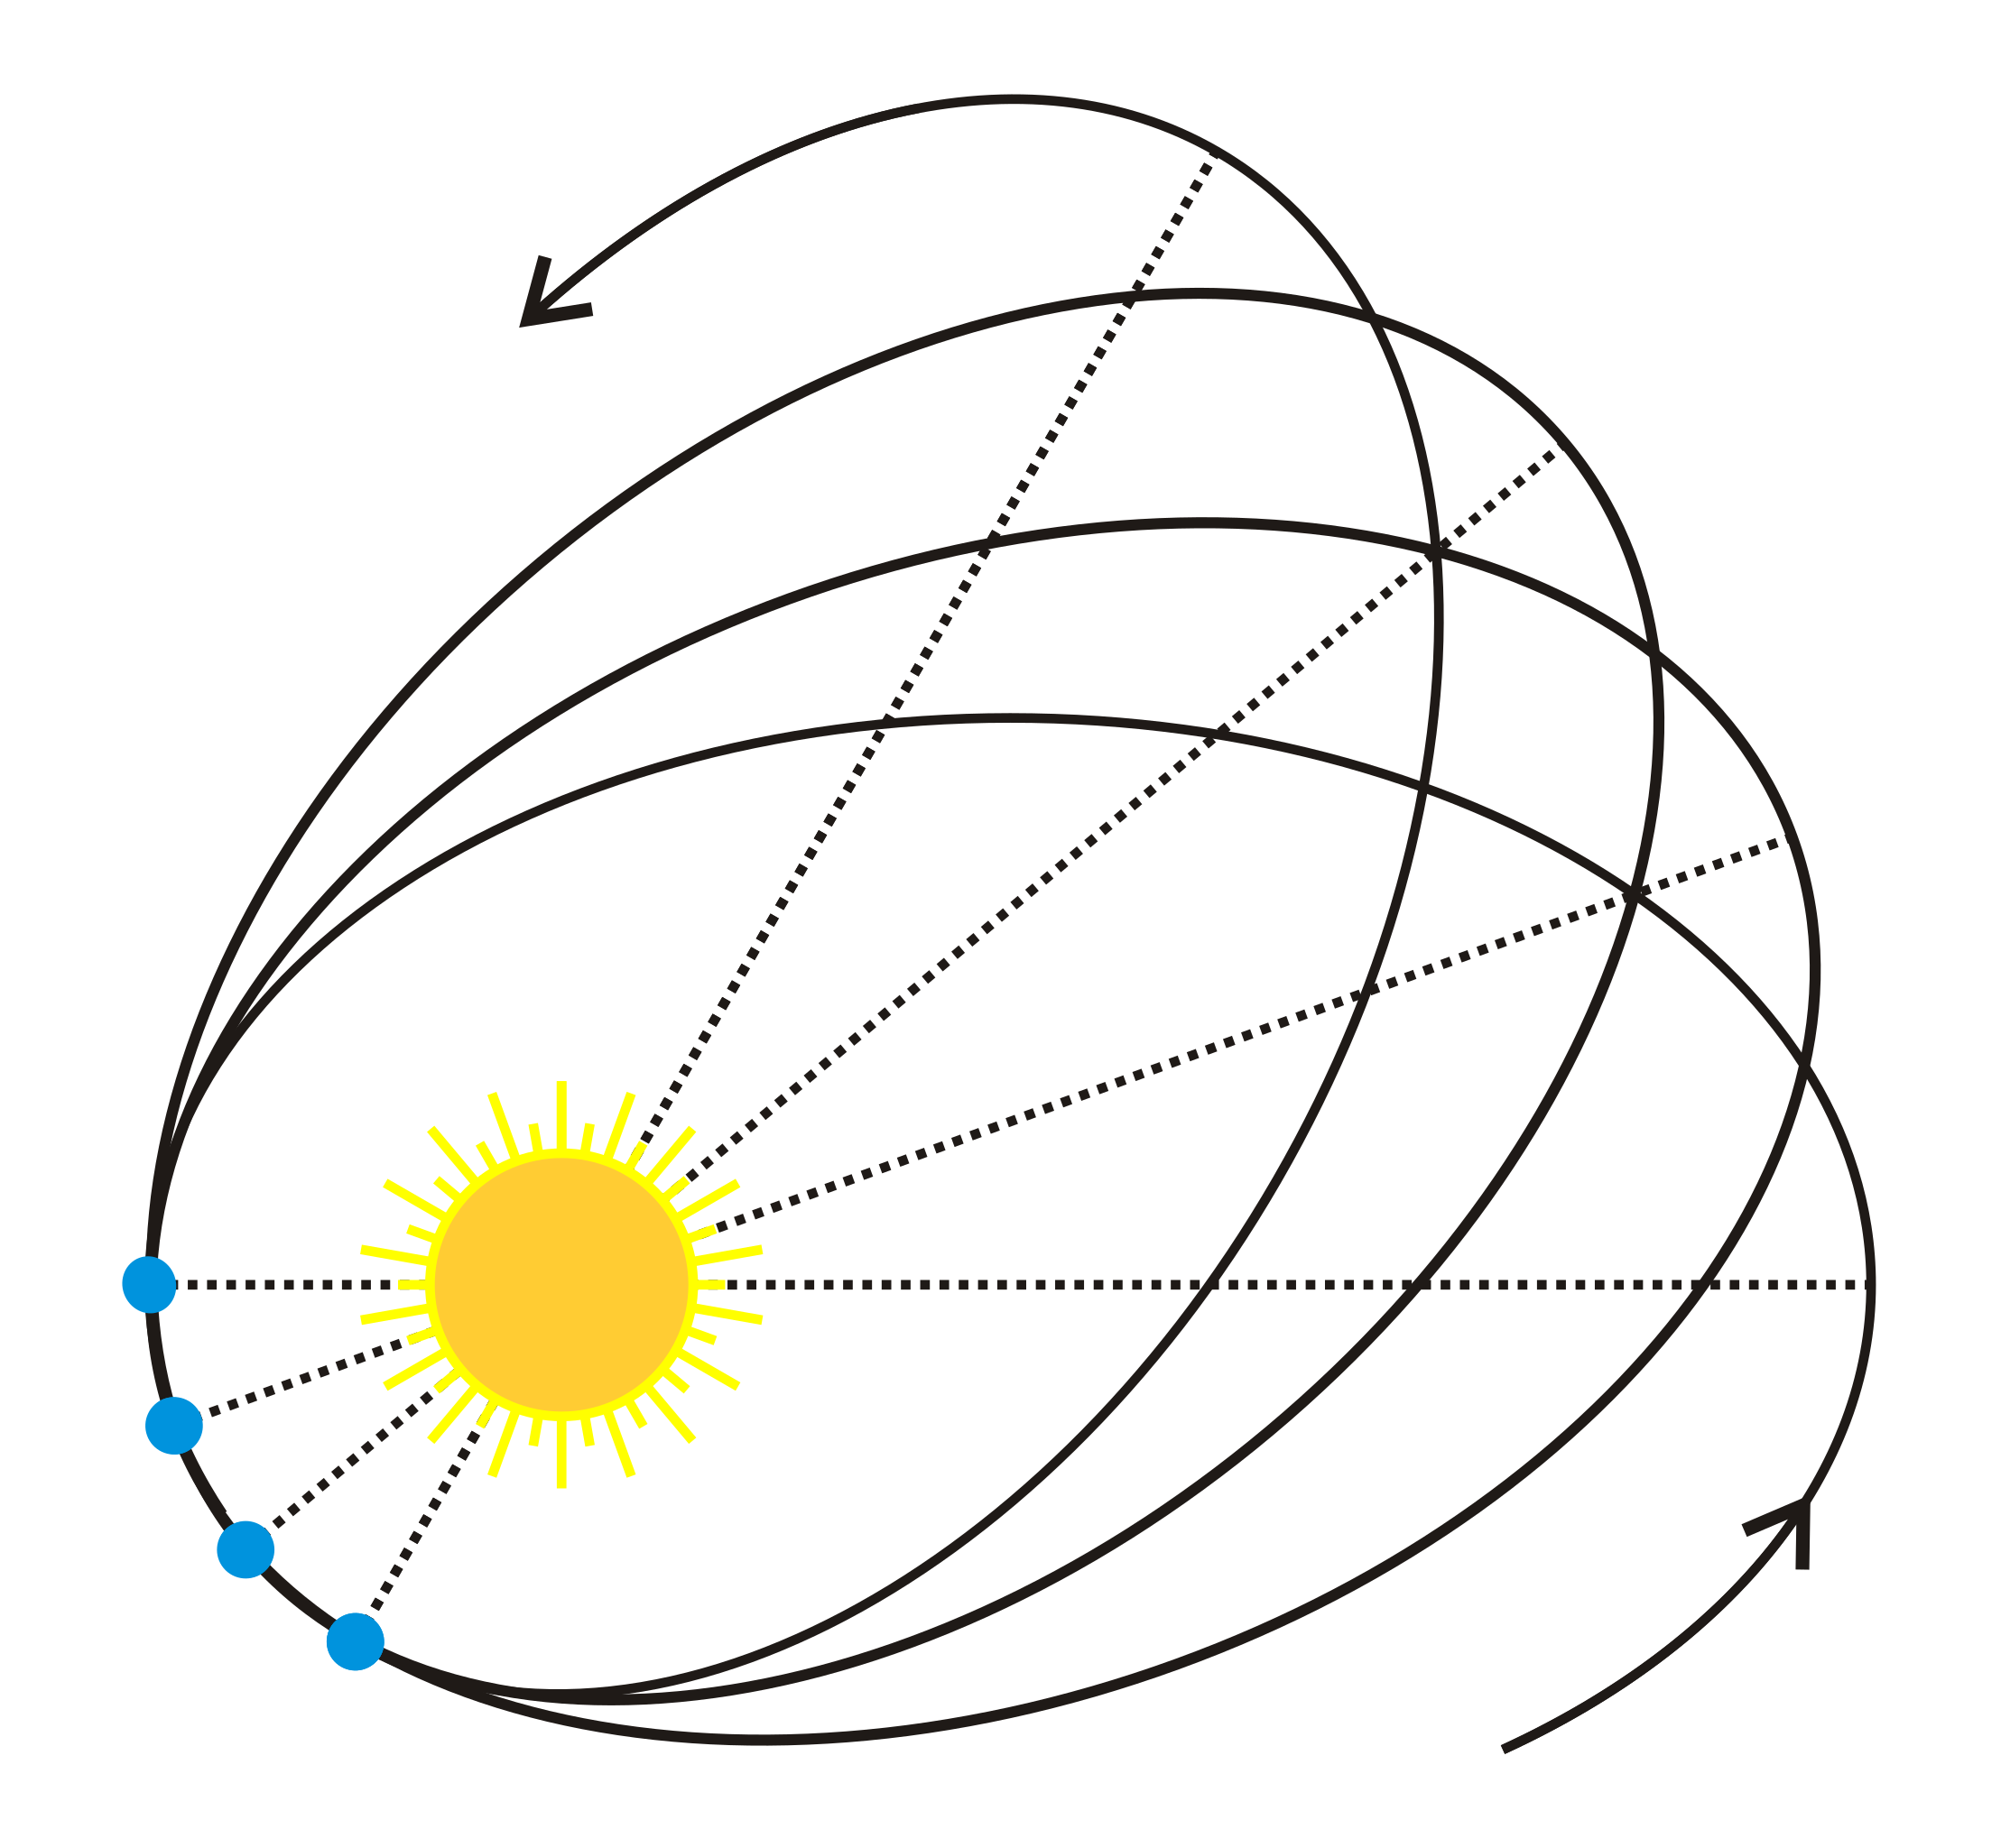
\includegraphics[width=1\textwidth]{Figures/Perihelion_precession2.png}
\caption{Precession of the perihelion of Mercury. Image taken from \cite{Perihelion_precession}}
\label{Perihelion_precession2}
\end{center}
\end{figure}

 


\chapter{Theoretical Framework}

In this section we are going to review the theoretical concepts on which the probabilistic methods here used are based. We will expose them following the approaches of Murphy \cite{murphy2012machine},  Koller et al. \cite{koller2009probabilistic}, H{\o}jsgaardand \cite{hojsgaard2012graphical} et al.  and Russel et al. \cite{russell2010artificial}.  Furthermore we will provide also a rapid overview about the main concepts of information theory,  following the Cover \cite{cover2006elements} and MacKay \cite{mackay2003information} approaches,  since we used some of its concepts in the preliminary analysis of the dataset. Finally this chapter will be concluded with a rapid overview about the concept of algorithm intepretability. Such concept, together with the accuracy and the confusion matrix, is necessary for the assessment of a ML performances. On the other side the concepts related to the celestial mechanics here used will be described, following the Murray approach \cite{murray1999solar} into the Appendix A

\section{Markov random fields}

Lets start by supposing that we would represent compactly a joint distribution such as \cite{murphy2012machine}:
\begin{equation}
p(x_{1},x_{2},...,x_{n})
\end{equation}
that can represent for instance words in a documents or pixels of an image.  Firstly we know that using the chain rule,  we can decompose it, into the following form \cite{murphy2012machine}:
\begin{equation}
p(x_{1:V})=p(x_{1})p(x_{2}|x_{1})p(x_{3}|x_{2},x_{1})...p(x_{V}|x_{1:V-1})
\end{equation}
where V is the number of variables and 1:V stands for ${1,2,...,V}$.  This decomposition makes explicit the conditional probability tables, or in other terms the transition probability tensors \cite{wu2017markov}.  As one can point out, the number of parameters is cumbersome as the number of variables grows: indeed the number of parameter required scales as $\mathcal{O}(K^{V})$.  Such formidable problem can be attacked by considering the concept of conditional independence. This is defined as\cite{murphy2012machine}:

\begin{equation}
X  \perp Y| Z \iff  p(X,Y|Z) = p(X|Z)p(Y|Z)
\end{equation}

A particular case of this definition is the Markov assumption,  by which \textit{the future is independent from the past given the present } or in symbols \cite{murphy2012machine}: 

\begin{equation}
p(\textbf{x}_{1:V})=p(x_{1})\prod^{V}_{t=1}p(x_{t}|x_{t-1})
\end{equation}

In this case a first order Markov chain is obtained,  where the transition tensor is of second order \cite{wu2017markov}.  Given this formalism we are interested in finding a smart way to plot such joint distribution into an intuitive way: the graph theory provide the answer to this quest.  In particular the random variables can be represented by nodes and presence of conditional independence for two random variables by the lack of an edge that interconnects them.  Bayesian networks consider directed edges,  while Markov random fields (MRF) only undirected.  As consequence,  while the the concept of topological ordering,  by which the parents n nodes are labelled with a lower  with respect to their children,  is well defined for Bayesian network,  for MRF is not.  In order to solve this issue it is useful to consider the Hammersley-Clifford theorem as stated in \cite{murphy2012machine}:

\begin{theorem}[Hammersley-Clifford]
A positive distribution p(\textbf{y})>0 satisfies the CI properties of an indirect graph G iif p can be represented as a product of factor, one per maximal clique,  i.e.
\begin{equation}
p(\textbf{y}|\theta)= \dfrac{1}{Z(\theta)}\prod_{c \in C }\psi_{c}(\textbf{y}_{c}|\theta_{c})
\end{equation}
where C is the set of all the (maximal) cliques of G,  and Z($\theta$) is the partition function given by 
\begin{equation}
Z(\theta):= \sum_{y}\prod_{c\in C}\psi_{c}(\textbf{y}_{c}|\theta_{c})
\end{equation}
Note that this partition function is what ensures the overall distribution sums to 1
\end{theorem}

Such theorem allows to represent a probability distribution with potential functions for each maximal clique in the graph.  A particular case of these is the Gibbs distribution \cite{murphy2012machine}: 

\begin{equation}
p(y|\theta)=\dfrac{1}{Z(\theta)} exp\left(-\sum_{c}E(y_{c}|\theta_{c})\right)
\end{equation}

where $E(y_{c})>0$ represent the energy associated with the variables in the clique c.  This form can be adapted to a UGM with the following expression \cite{murphy2012machine}:

\begin{equation}
\psi_{c}(y_{c}|\theta_{c})=exp\left(-E(y_{c}|\theta_{c})\right)
\end{equation}

Finally in order to reduce the computational cost,  one can consider only the pairwise interaction instead of the maximum clique. This is the analogue of what is usually performed in solid state physics (but surely not always)  when only the interaction between the first neighbour is considered.  Another example is the  Ising model: here we have a lattice of spins that can be or in $\ket{+}$ or in $\ket{-}$ and their interaction is modelled by\cite{murphy2012machine}:


\begin{equation}
\psi_{st}\left(y_{s},y_{t}\right) =
\begin{pmatrix}
e^{w_{st}} & e^{-w_{st}} \\
e^{-w_{st}} & e^{w_{st}} \\
\end{pmatrix}
\end{equation}

where $w_{st}=J$ represent the coupling strength between two neighbour site.  The collective state is described by 

\begin{equation}
\ket{i_{1},i_{2},...,i_{n}}=\ket{i_{1}}\otimes\ket{i_{2}}\otimes...\otimes\ket{i_{n}}
\end{equation}

where $\otimes$ is the tensor product.  If this parameter is associated with a positive finite value we have an associative Markov network: basically collective states in which all sites have the same configuration is favoured. Thus we will have two collective states: one for which we have all $\ket{+}$ and another in which we have all $\ket{-}$  Such situation would model,  in principle,  the ferromagnet materials where the external magnetic field induce into the material a magnetic filed with the same direction.  On the other side if the magnetization of the material is opposite with respect to the external field,  and thus $J<0$,  we have an anti-ferromagnetic system in which frustrated states are present.  Furthermore lets consider the unnormalized log probability of a collective state $\textbf{y}=\ket{i_{1},i_{2},...,i_{n}}$ \cite{murphy2012machine}:

\begin{equation}
\log\tilde{\textbf{p}}(y)= -\sum_{s\sim t}y_{s}w_{st}y_{t}
\end{equation}

If we also consider an external field \cite{murphy2012machine}:

\begin{equation}
\log\tilde{\textbf{p}}(y)= -\sum_{s\sim t}y_{s}w_{st}y_{t}+\sum_{s}b_{s}y_{s}
\end{equation}

But this is nothing more that the well know \footnote{In physics} Hamiltonian of an Ising system. This is not a simple coincidence:  indeed the Hamiltonian of a system represent,  rudely speaking,  its total energy.  Thus according to the Boltzmann or Gibbs distribution we have \cite{murphy2012machine}:

\begin{equation}
P_{\beta}(\textbf{y})=\dfrac{e^{-\beta H(\textbf{y}})}{Z_{\beta}}
\end{equation}

where $\beta$ is proportional to the inverse of the system temperature.  Coming back the unnormalized probability of a collective state $\textbf{y}$,  if we set $\Sigma^{-1}=\textbf{W}$,  $\boldsymbol{\mu}=\boldsymbol{\Sigma} \textbf{b}$ and $c=\dfrac{1}{2}\mu^{T}\boldsymbol{\Sigma}^{-1}\mu$ we obtain a Gaussian \cite{murphy2012machine}:

\begin{equation}
\tilde{\textbf{p}}(y)\sim exp\left( -\frac{1}{2} (\textbf{y}-\boldsymbol{\mu})^{T} \boldsymbol{\Sigma}^{-1} (\textbf{y}-\boldsymbol{\mu}) + c \right)
\end{equation}

In general we refer to Gaussian Markov random fields for a joint distribution that can be decomposed in the following way \cite{murphy2012machine}:

\begin{equation}
p\left(\textbf{y}|\boldsymbol{\theta}\right) \propto \prod_{s\sim t} \psi_{st}\left(y_{s},y_{t}\right)\prod_{t}\psi_{t}\left(y_{t}\right)
\end{equation}

\begin{equation}
\psi_{st}\left( y_{s},y_{t} \right)=exp\left( -\dfrac{1}{2} y_{s}\Delta_{st}y_{t} \right)
\end{equation}

\begin{equation}
\psi_{t}\left(y_{t}\right)= \exp \left( -\dfrac{1}{2}\Delta_{tt}y^{2}_{t}+\eta_{t}y_{t}\right)
\end{equation}

\begin{equation}
p\left(\textbf{y}|\boldsymbol{\theta}\right) \propto \exp \left( \boldsymbol{\eta}^{T} \textbf{y}-\dfrac{1}{2}y^{T}\Delta \textbf{y} \right)
\end{equation}

(this last expression can be reconducted to the multivariate gassian if one consider $\boldsymbol{\Delta}=\boldsymbol{\Sigma}^{-1}$ and $\boldsymbol{\eta}=\boldsymbol{\Delta}\boldsymbol{\mu}$. Given the network, we would now move on how the parameters can be achieved. Lets start from a Markov random field in log-linear form \cite{murphy2012machine}:

\begin{equation}
p\left(\textbf{y}|\boldsymbol{\theta}\right) = \dfrac{1}{Z(\theta)}\exp \left( \sum_{c}\boldsymbol{\theta}^{T}_{c}\phi_{c}\left(\textbf{y}\right)\right)
\end{equation}

thus we can define the log-likehood as \cite{murphy2012machine}:

\begin{equation}
\mathcal{L}\left(\boldsymbol{\theta}\right):= \frac{1}{N}\sum_{i}\log p\left(\textbf{y}_{i}|\boldsymbol{\theta}\right)=\frac{1}{N}\sum_{i}\left[\sum_{c} \boldsymbol{\theta}^{T}_{c}\phi_{c}(y_{i})-\log Z\left(\boldsymbol{\theta}\right)\right]
\end{equation}

\begin{equation}
\frac{\partial\mathcal{L}}{\partial\boldsymbol{\theta}_{c}}=\frac{1}{N}\sum_{i}\left[\phi_{c}(y_{i})-\frac{\partial}{\partial\boldsymbol{\theta}_{c}}\log Z(\boldsymbol{\theta})\right]
\end{equation}

\begin{equation}
\frac{\partial \log Z(\boldsymbol{\theta})}{\partial\boldsymbol{\theta}}=\mathbb{E}\left[\phi_{c}(\textbf{y})\right|\theta]=\sum_{\textbf{y}}\phi_{c}(\textbf{y})p(\textbf{y}|\boldsymbol{\theta})}
\end{equation}


\begin{equation}
\frac{\partial\mathcal{L}}{\partial\boldsymbol{\theta}_{c}}=\left[\frac{1}{N}\sum_{i}\phi_{c}(y_{i})\right]-\mathbb{E}\left[\phi_{c}(\textbf{y})\right]
\end{equation}

In the first term $\textbf{y}$ is fixed to its observed values while in the second it is free. Such expression can be recasted in to a more explicative form \cite{murphy2012machine}:

\begin{equation}
\frac{\partial\mathcal{L}}{\partial\boldsymbol{\theta}_{c}}=\mathbb{E}_{p_{emp}}\left[\phi_{c}(\textbf{y})\right]-\mathbb{E}_{p_{(\cdot|\boldsymbol{\theta})}}\left[\phi_{c}(\textbf{y})\right]
\end{equation}

Therfore at the optimum we will have \cite{murphy2012machine}:

\begin{equation}
\mathbb{E}_{p_{emp}}\left[\phi_{c}(\textbf{y})\right]=\mathbb{E}_{p_{(\cdot|\boldsymbol{\theta})}}\left[\phi_{c}(\textbf{y})\right]
\end{equation}

From this expression it is clear why this method is called moment matching; it is worth nothing tha such computation is largely expensive from a computational point of view: thus scholar usually consider other techinques or at least stochastic gradient descent method. A full review can be found in \cite{murphy2012machine} and \cite{koller2009probabilistic}. Finally we consider, as for the dataset in analysed in this work, the case where we have both discrete and continuous variables i.e. $x=\left(i_{1},...,i_{d},y_{1},...,y_{q} \right)$ with d discrete variable and q continuos variables. The are called in the literature Mixed Interaction Models. In this case the following density has to be considered \cite{hojsgaard2012graphical}:

\begin{equation}
\begin{split}
f(i,y)=& p(i)(2\pi)^{-q/2}det(\Sigma)^{-1/2} \\
& exp\left[-\dfrac{1}{2}\left(y-\mu(i)\right)^{T}\Sigma^{-1}\left(y-\mu(i)\right)\right]
\end{split}
\label{gaussMix}
\end{equation}

Which can be rewritten in the exponential family form \cite{hojsgaard2012graphical}: 

\begin{equation}
\begin{split}
f(i,y) & = \exp\left\lbrace g(i)+\sum_{u}h^{u}(i)y_{u}-\dfrac{1}{2}\sum_{uv} y_{u}y_{v}k_{uv}\right\rbrace \\
&= \exp\left\lbrace g(i)+h(i)^{T}y-\dfrac{1}{2}y^{T}Ky \right\rbrace
\end{split}
\end{equation}

where $g(i)$, $h(i)$ and $K$ are the canonical parameters. These are connected with the parameters of expression \ref{gaussMix} by the following identities \cite{hojsgaard2012graphical}: 

\begin{equation}
\begin{split}
K=&\Sigma^{-1} \\
h(i)=&\Sigma^{-1}\mu(i) \\
g(i)=&\log p(i) -\frac{1}{2}\log det (\Sigma) \\
&-\dfrac{1}{2}\mu(i)^{T}\Sigma^{-1}\mu(i)-\dfrac{q}{2}\log 2\pi
\end{split}
\end{equation}

Moreover one can further modify the previous form in order to obtain a particular factorial expansion: such models are referred as homogeneous mixed interaction models \cite{hojsgaard2012graphical}.

\section{Information theory}
Given an ensemble of random variable, we can qunaitify the amount of information that one variable contains of another one: such quantity is called mutual information and it is a key concept within the information theory. This approach, that was implemented by Claude Shannon decades before the probabilistic modelling, represent a complementary way by which one can attack the problem of conditional dependence between random variables. Here we would provide some basic concepts of this theory, following the Cover \cite{cover2006elements} and MacKay \cite{mackay2003information} approaches, that allow to properly define the concept of mutual information. The founding concept of information theory is the entropy. This quantity express the uncertainty of a random variable. Given a random variable $X$ with alphabet (the accessible states) $\cite{cover2006elements}$ and probability mass function $p(x)=Pr\left\lbrace X=x \rbrace\; x \in \chi$ we define the entropy of $X$ as $H(X)=-\sum_{x \in X} p(x)log p(x)$ where the logarithm has to be considered with basis 2. In analogous way the joint entropy of two random variables $(X,Y)$ with a joint distribution p(x,y) is defined as \cite{cover2006elements}:
\begin{equation}
H(X,Y)=-\sum_{x\in \chi}\sum_{y\in \mathcal{Y}}p(x,y)\log p(x,y)
\end{equation}
Furthermore, we can define also the conditional entropy as \cite{cover2006elements}:
\begin{equation}
\begin{split}
H(X|Y)=& \sum_{x\in \mathcal{X} }p(x)H(Y|X=x)\\
=& -\sum_{x\in \mathcal{X}}p(x)\sum_{y\in \mathcal{Y}}p(x,y)\log p(y|x) \\
=& -E\log p(Y|X)
\end{split}
\end{equation}
The joint entropy and the conditional entropy are related by the chain rule \cite{cover2006elements}:
\begin{equation}
H(X,Y)=H(X)+H(Y|X)
\end{equation}
Such rule can be extended to to the following from \cite{cover2006elements}:
\begin{equation}
H(X,Y|Z)=H(X|Z)+H(Y|X,Z)
\end{equation}
Given a distribution q and another distribution p, one can quantify how inefficently the second one describe the first one using the concept of relative entropy or Kullback-Leibler distance \cite{cover2006elements,mackay2003information}:
\begin{equation}
D(p||q)=\sum p(x)\log\frac{p(x)}{q(x)}
\end{equation}
As stated by the Gibbs inequality \cite{cover2006elements,mackay2003information}:
\begin{equation}
D(p||q)\geq 0
\end{equation}
this quantity can not be negative: the entropy of a random variable associated to another cannot have a degree of uncertainty lower with respect to the quantity that its aimed to describe. On these basis we are now ready to introduce the concept of mutual information. This is defined as  \cite{cover2006elements}:
\begin{equation}
\begin{split}
I(X;Y)&=\sum\sump(x,y)\log\dfrac{p(x,y)}{p(x)p(y)}=\\
&=D(p(x,y)||p(x)p(y)) \\
&=H(X)-H(X|Y)=H(Y)-H(Y|X)
\end{split}
\end{equation}
As for the joint distribution also in this case we have a chain rule  \cite{cover2006elements}:
\begin{equation}
I(X_{1},X_{2},...,X_{n};Y)=\sum^{n}_{i=1}I(X_{i};Y|X_{i-1},X_{i-2},...,X_{1})
\end{equation}
Finally we would report the data process inequality theorem that connects the information theory with the Markov chain: if we have a Markov chains, $X\rightarrow Y \rightarrow Z$  then $I(X;Y)\geq I(X;Z) $. As for the Gibbs inequality, the underlying idea is that no clever manipulation of the data can improve the inference that can be made on them \cite{cover2006elements,mackay2003information}. Otherwise we would have a clear violation of the second principle of thermodynamics (see for instance the Maxwell's demon \cite{feynman2018feynman})

\section{Algorithm intepretability}

Beside the accuracy and other features that are connected with the confusion matrix, another important feature is the algorithm intepretability. This feature, at a first instance, is connected on how much the algorithm provide explanation to a human on how it choose a forecast instead of another one, or in other word how much the algorithm is not a blackbox. Apart from all legal problems connected with an algorithm that is a blackbox\footnote{Think for instance the conditions imposed by the GDPR (e.g the right to explanation)}, in the author opinion results provided by such algorithm cannot be considered scientific, since the scientific method also requires to provide an explanation and not simply almost correct forecast. Following the Tarski et al. \cite{tarski1953undecidable} argument, which is based on mathematical logic, it can be said that the a formal theory T can be translated into S if and only if S is able to proof the theorem of T in its own language. On the other side we would also that an algorithm, as an explanation, is complete: we expect that it will be also able to make correct forecasts for all available data. However as shown by \cite{doshi2017towards} and by \cite{gilpin2018explaining} the intepretability of an algorithm is linked with its incompleteness. This is something that is nested both in formal system as algorithms or scientific theories. For instance lets consider the fall of object: at first glance one can consider the only the items on Earth, in this case the acceleration is constant and it is a very simple theory; but as one moves to consider also the interaction within planets a much more complicate law should be considered (in which the previous case is a particular one). The first one is fully explainable but poorly complete, the second one more difficult to explain but much more complete. Therefore, in principle, the evaluation of an algorithm performances should be considered not only in to one dimension, the accuracy, but also by considering its intepretability as shown in Fig. \ref{ML_intepretability}

\begin{figure}[h]
\begin{center}
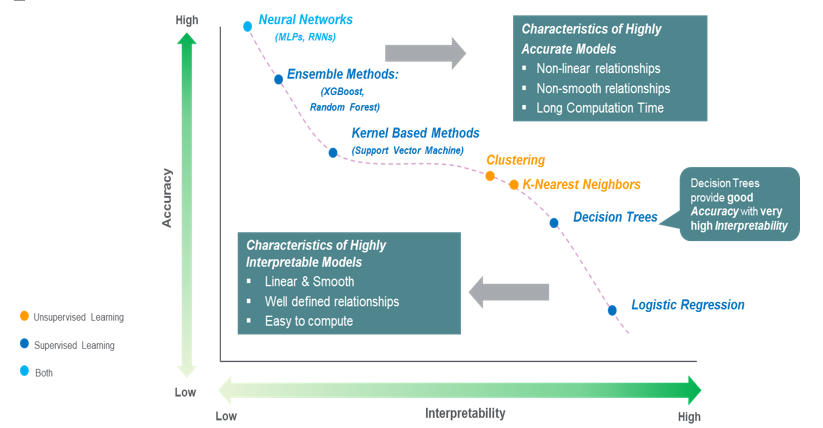
\includegraphics[width=1\textwidth]{Figures/ML_intepretability.png}
\caption{Different ML algorithms classified by their interpretability and by their accuracy. Image taken from \cite{ml_interpretability}}
\label{ML_intepretability}
\end{center}
\end{figure}


\chapter{Dataset description}

The asteroid dataset was retrieved from Kaggle \cite{kaggle_dataset}, which reports into an more user-friendly mode the dataset of The Center for Near-Earth Object Studies (CNEOS) \cite{cneos+nasa}, a NASA research center. Among the 40 features that were present in the dataset we excluded the ones that were clearly redundant (such as the distance quantity evaluated in miles instead of kilometres), the ones that were connected only to the other name of the asteroid, the one connected to the name of the orbit and the one connected with the orbiting planet, since for all it was the Earth. Thus the features obtained were therefore reduced to 22. Their description will be postponed to Appendix A, since a description of them cannot be disjoint with celestial mechanics concepts. Their enumeration is provided in Tab. \ref{tab_features}. Since only the 16 \% of the asteroids were hazardous, we considered to reduce the number of the non-hazardous in order to improve the portion of the hazardous ones. For this purpose we constructed a database in which the proportion hazardous/not hazardous was 1:5: thus all the hazardous one were included, while the not-hazardous were randomly selected \footnote{The author is aware that in principle the proportion should be much less unbalanced, however the tool that has to be paid for this operation is an overall reduction of the cases in the dataset that lowers the performances of the algorithms here used. The proportion here used was a trade-off for these two contrasting facts}. Furthermore, concerning the continuous measures, the dataset was standardised and demeaned. 


\begin{table}[]
\caption{The features used for the present analysis. The unit of measure are reported in the original dataset \cite{kaggle_dataset}.}
\begin{center}
\begin{tabular}{c|c}
\hline
\textbf{Features}             & \textbf{Type}        \\ \hline
Neo Reference ID              & not used             \\ \hline
Absolute Magnitude            & Continuous           \\ \hline
Est Dia in KM (min)           & Continuous           \\ \hline
Est Dia in KM (max)           & Continuous           \\ \hline
Close Approach Date           & Continuous           \\ \hline
Epoch Date Close Approach     & Continuous           \\ \hline
Relative\_Velocity            & Continuous           \\ \hline
Miss\_Dist                    & Continuous           \\ \hline
Min\_Orbit\_Intersection      & Continuous           \\ \hline
Jupiter\_Tisserand\_Invariant & Continuous           \\ \hline
Epoch\_Osculation             & Continuous           \\ \hline
Eccentricity                  & Continuous           \\ \hline
Semi Major Axis               & Continuous           \\ \hline
Inclination                   & Continuous           \\ \hline
Asc Node Longitude            & Continuous           \\ \hline
Orbital Period                & Continuous           \\ \hline
Perihelion Distance           & Continuous           \\ \hline
Perihelion Arg                & Continuous           \\ \hline
Perihelion Time               & Continuous           \\ \hline
Mean\_Anomaly                 & Continuous           \\ \hline
Mean\_Motion                  & Continuous           \\ \hline
Hazardous                     & Categorical (Binary)
\end{tabular}
\end{center}
\label{tab_features}
\end{table}


\chapter{Results and discussion}

This chapter is organized in the following way: first we are going to report the results concerning the preliminary analysis performed on the dataset. This include the factor analysis of mixed data and the mutual information analysis of the continuous variables of asteroids vs their hazard. Then it will follow the analysis of the dataset performed with the probabilistic methods: after a preliminary analysis on the continuous variables, the mixed interaction model as well the minforest model obtained for the whole dataset will be presented and discussed. Finally the probabilistic models previously obtained will be compared with the outputs and the performances of four machine learning algorithm (Random Forest, Support vector machines Quadratic Discriminant Analysis and Logistic regression).

\section{Preliminary analysis}

The first inspection that was performed on the dataset was related to the density distributions of a selection of continuous features that are known, from the celestial mechanics, to be important for the prediction of the asteroids dangerousness. These are reported in Fig. \ref{Density_relevant}. Next we moved on a more systematic analysis with FADM and mutual information. In Fig. \ref{FADM},\ref{FAMD_Quantitative variables} and \ref{FAMD_Individuals_(c)} are reported the main achivements of FADM (performed with FactoMineR package \cite{le2008factominer}): in particular from the correlation circle in Fig. \ref{FAMD_Quantitative variables} the different correlations that are given by the celestial mechanics laws can be recognized: for instance, see that there is strong correlation of the mean motion with the semi-major axis. This is due to the Kepler law discussed in Appendix A. Furthermore we see that that the mean motion is correctly almost independent with respect to the the diameter (max or min) of  the asteroid. As explained in Appendix A this is an another result of Newton gravitation theory for a two body interaction: the mean motion of an asteroid, as long as the the mass of it is much lower with respect to the sun, is independent from its mass. On the other side the fact that relative velocity is correlated with the diameter is a spurios correlation. At this point one can ask why the mean motion and the relative velocity are orthogonal: this point will be clarified from a theoretical point of view in appendix A and also with graphical models. Briefly the motion of an object on an ellipse as seen from a focus is not uniform: this is faster as the two bodies approaches. Beside this inspection a further analysis based on the concept of mutual information (summarized in the previous chapter) was performed: its result is reported in Fig. \ref{Mutual_information}. This figure summarize the ranking of the features considered in the dataset for the dangerousness classification of the asteroids according to the following expression \cite{kratzer2018varrank}

\begin{equation}
g(\alpha,\textbf{C},\textbf{S},f_{i})=MI(f_{i};\textbf{C})-\sum_{f_{s}\in S}\alpha(f_{i},f_{s},\textbf{C},\textbf{S})MI(f_{i};f_{s})
\end{equation}
where the first term $MI(f_{i};\textbf{C})$ is called relevance and measures the Mutual Information between the interesting feature set $\textbf{C}$ (only Hazardous in our case) and the analysed one $f_{i}$; the third term $MI(f_{i};f_{s})$ is called redundancy and measures the MI between the analysed feature and a chosen set of them. Finally the $\alpha(f_{i},f_{s},\textbf{C},\textbf{S})$ is a normalization function and in our case was set to \cite{kratzer2018varrank}

\begin{equation}
\alpha(f_{i},f_{s},\textbf{C},\textbf{S})=\dfrac{1}{|\textbf{S}|}
\end{equation}

following the Peng. et al approach \cite{peng2005feature}. We see that the first place in the mutual information ranking, looking to the diagonal element, is taken by minimum orbit intersection: this is correct since this is one parameter used by NASA for deciding if an asteroid is hazardous or not (see Appendix A). The second place is occupied by Epoch date close approach. The third place is the eccentricity value: this parameter is entangled with the minimum orbit intersection and thus it is reasonable that it is important. Then we have two parameter that are related to the dimension of the asteroid: this is meaningful since if the asteroid has a too reduced volume it will be destroyed by the Earth atmosphere. On the other side the other parameters seems to have a too low MI for being interesting in this preliminary analysis. The results obtained for FAMD and MI will provide a useful path-guide, together with the celestial mechanics theory, for the interpretation of the results obtained in the following section 


\begin{figure}[ht]
  \begin{minipage}[b]{0.5\linewidth}
    \centering
    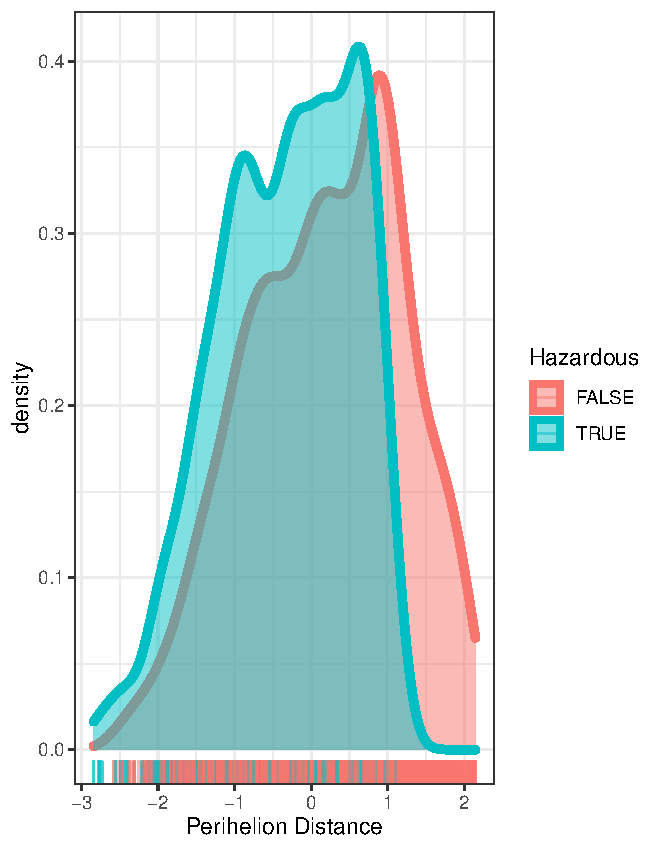
\includegraphics[width=.9\linewidth]{Figures/DENSITY_Perihelion_Distance.pdf}
    \subcaption{ \begin{center}
    a) Perihelion Distance
    \end{center}}
    \vspace{4ex}
  \end{minipage} 
  \begin{minipage}[b]{0.5\linewidth}
    \centering
    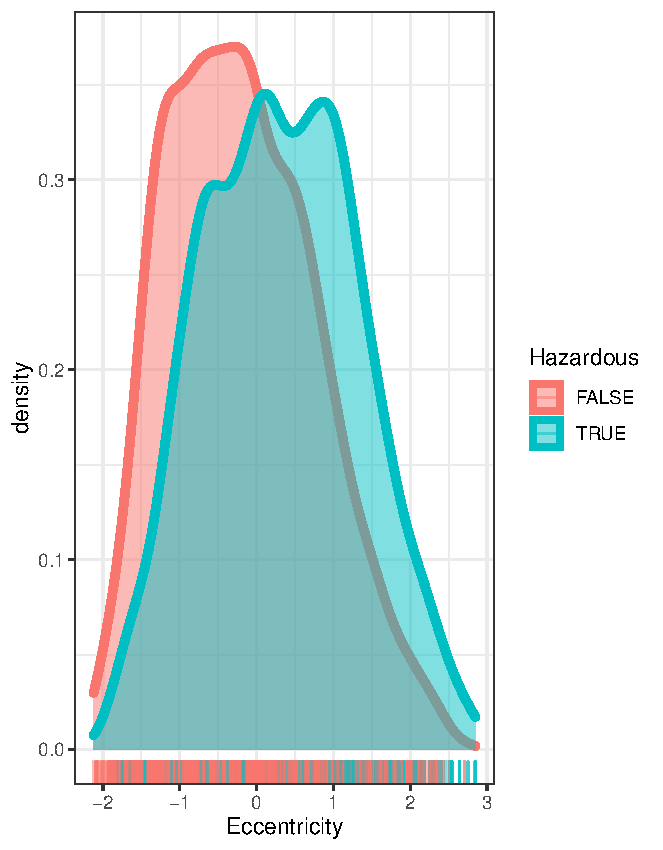
\includegraphics[width=.9\linewidth]{Figures/DENSITY_Eccentricity.pdf}
    \subcaption{ \begin{center}
    b) Eccentricity
    \end{center}}
    \vspace{4ex}
  \end{minipage} \\
    \begin{minipage}[b]{0.5\linewidth}
    \centering
    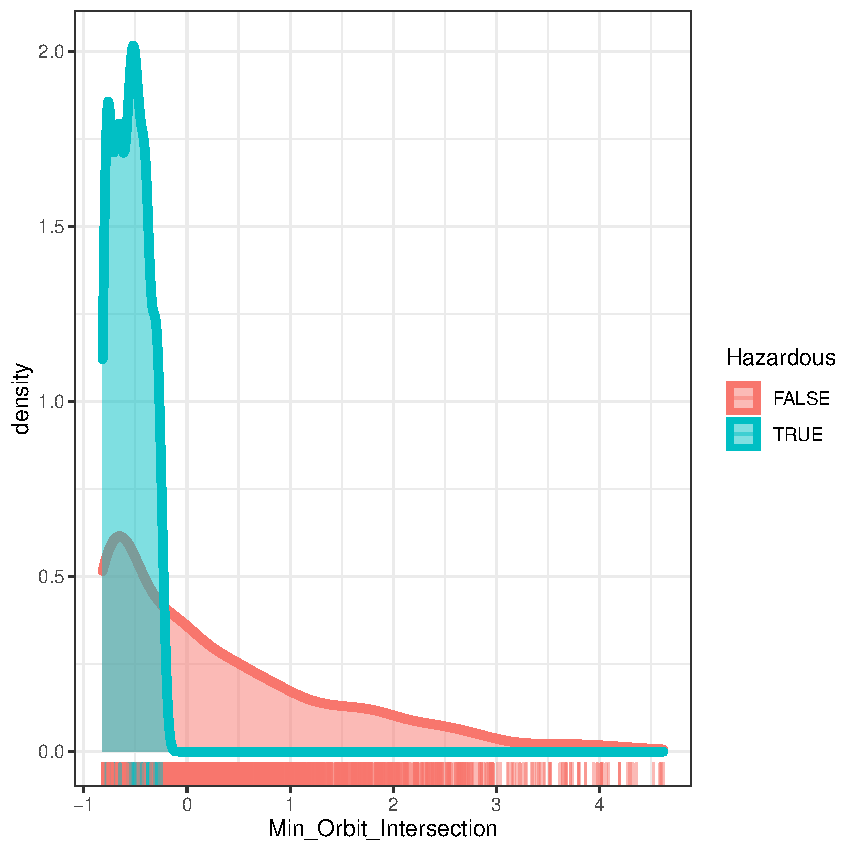
\includegraphics[width=.9\linewidth]{Figures/DENSITY_Min_orbit_intersection.pdf}
    \subcaption{ \begin{center}
    c) Min orbit intersection
    \end{center}}
    \vspace{4ex}
  \end{minipage}
  \begin{minipage}[b]{0.5\linewidth}
    \centering
    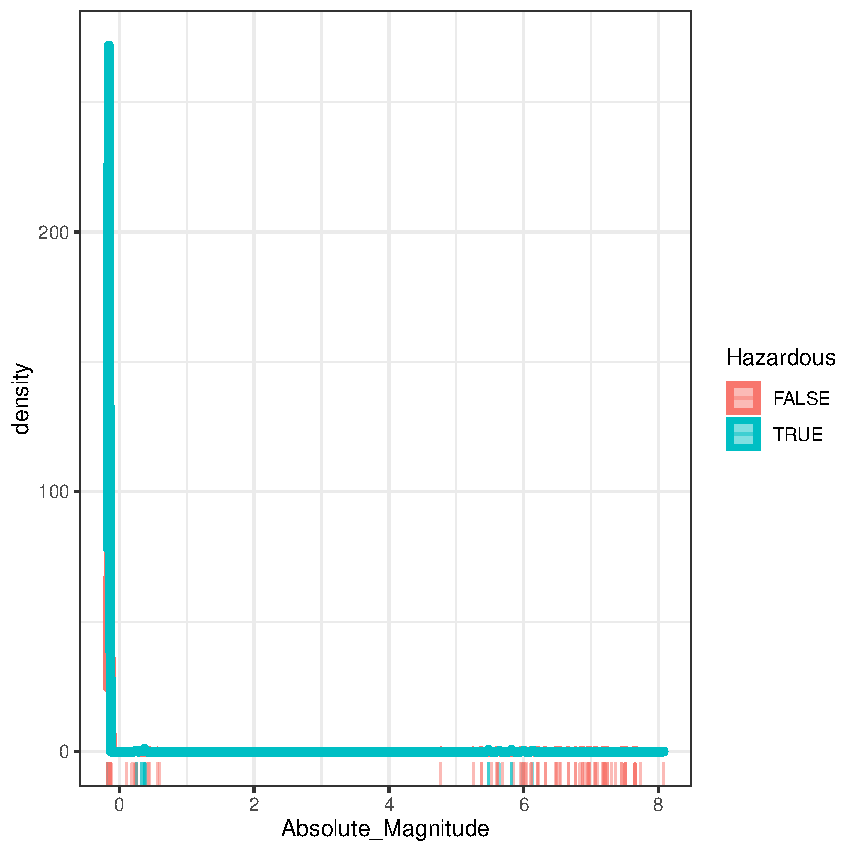
\includegraphics[width=.9\linewidth]{Figures/DENSITY_Absolute_magnitude.pdf}
    \subcaption{ \begin{center}
    d) Semi Major Axis
    \end{center}}
    \vspace{4ex}
  \end{minipage}
\caption{Comparison between the density distributions of hazardous (red) and non-hazardous (light blue) asteroids for a selected set of features that, according to the theory, are interesting.}
\label{Density_relevant}
\end{figure}


\begin{figure}[h]
\begin{center}
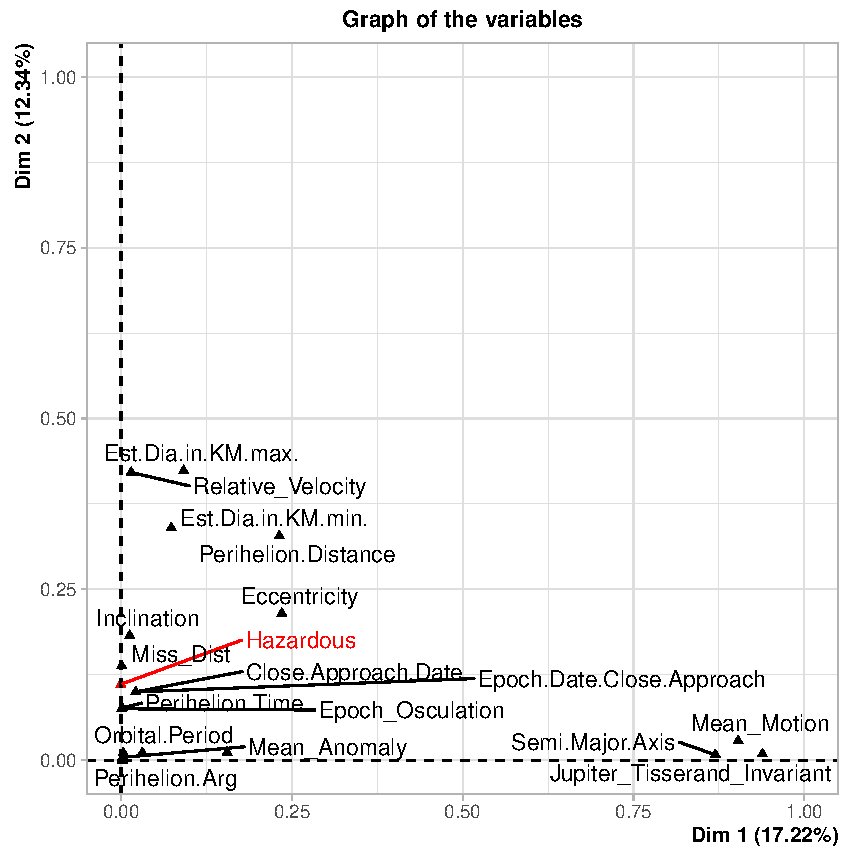
\includegraphics[width=1\textwidth]{Figures/FAMD.pdf}
\caption{The FAMD main plot in which the correlation between the continuous and discrete variables is reported. Plot obtained from FactoMineR package \cite{le2008factominer}}
\label{FADM}
\end{center}
\end{figure}

\begin{figure}[h]
\begin{center}
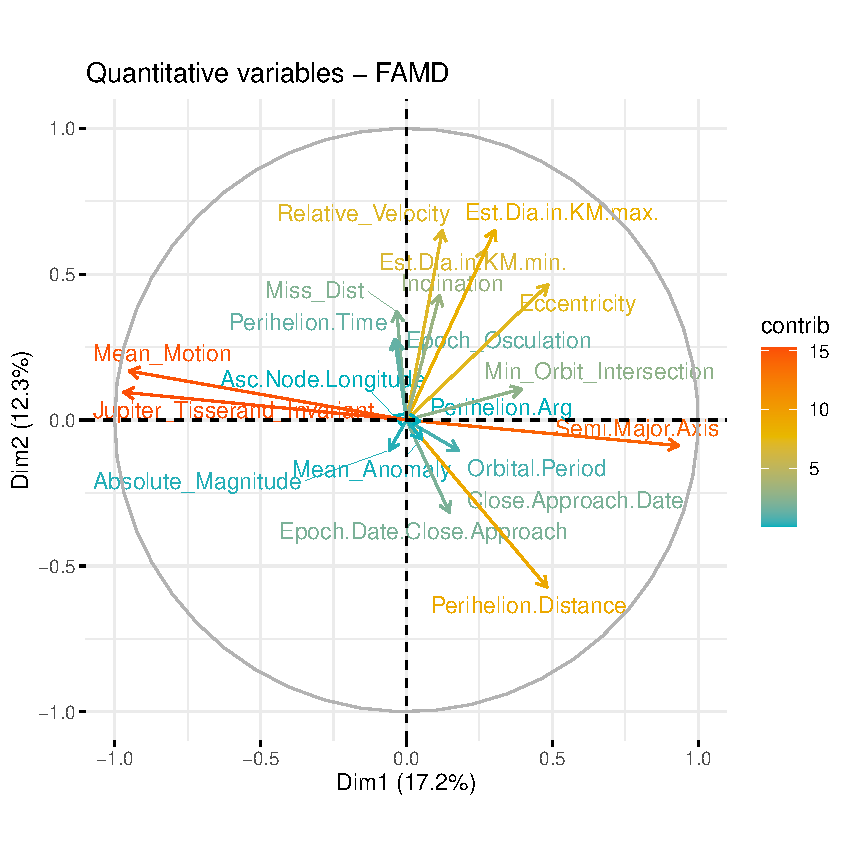
\includegraphics[width=1\textwidth]{Figures/FAMD_Quantitative variables.pdf}
\caption{The FAMD correlation circle for continuos variables as obtained from FactoMineR package \cite{le2008factominer}}
\label{FAMD_Quantitative variables}
\end{center}
\end{figure}

\begin{figure}[h]
\begin{center}
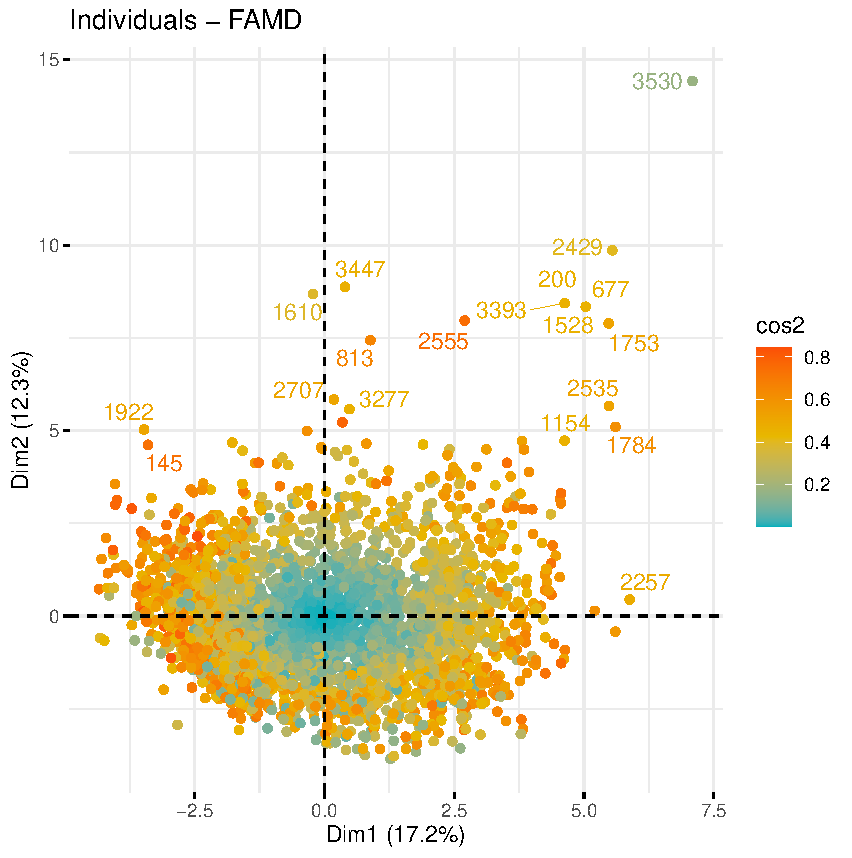
\includegraphics[width=1\textwidth]{Figures/FAMD_Individuals_(c).pdf}
\caption{Graph of individuals, for the qualititative variables, as obtained from FactoMineR package \cite{le2008factominer}}
\label{FAMD_Individuals_(c)}
\end{center}
\end{figure}

\begin{landscape}
\begin{figure}
\begin{center}
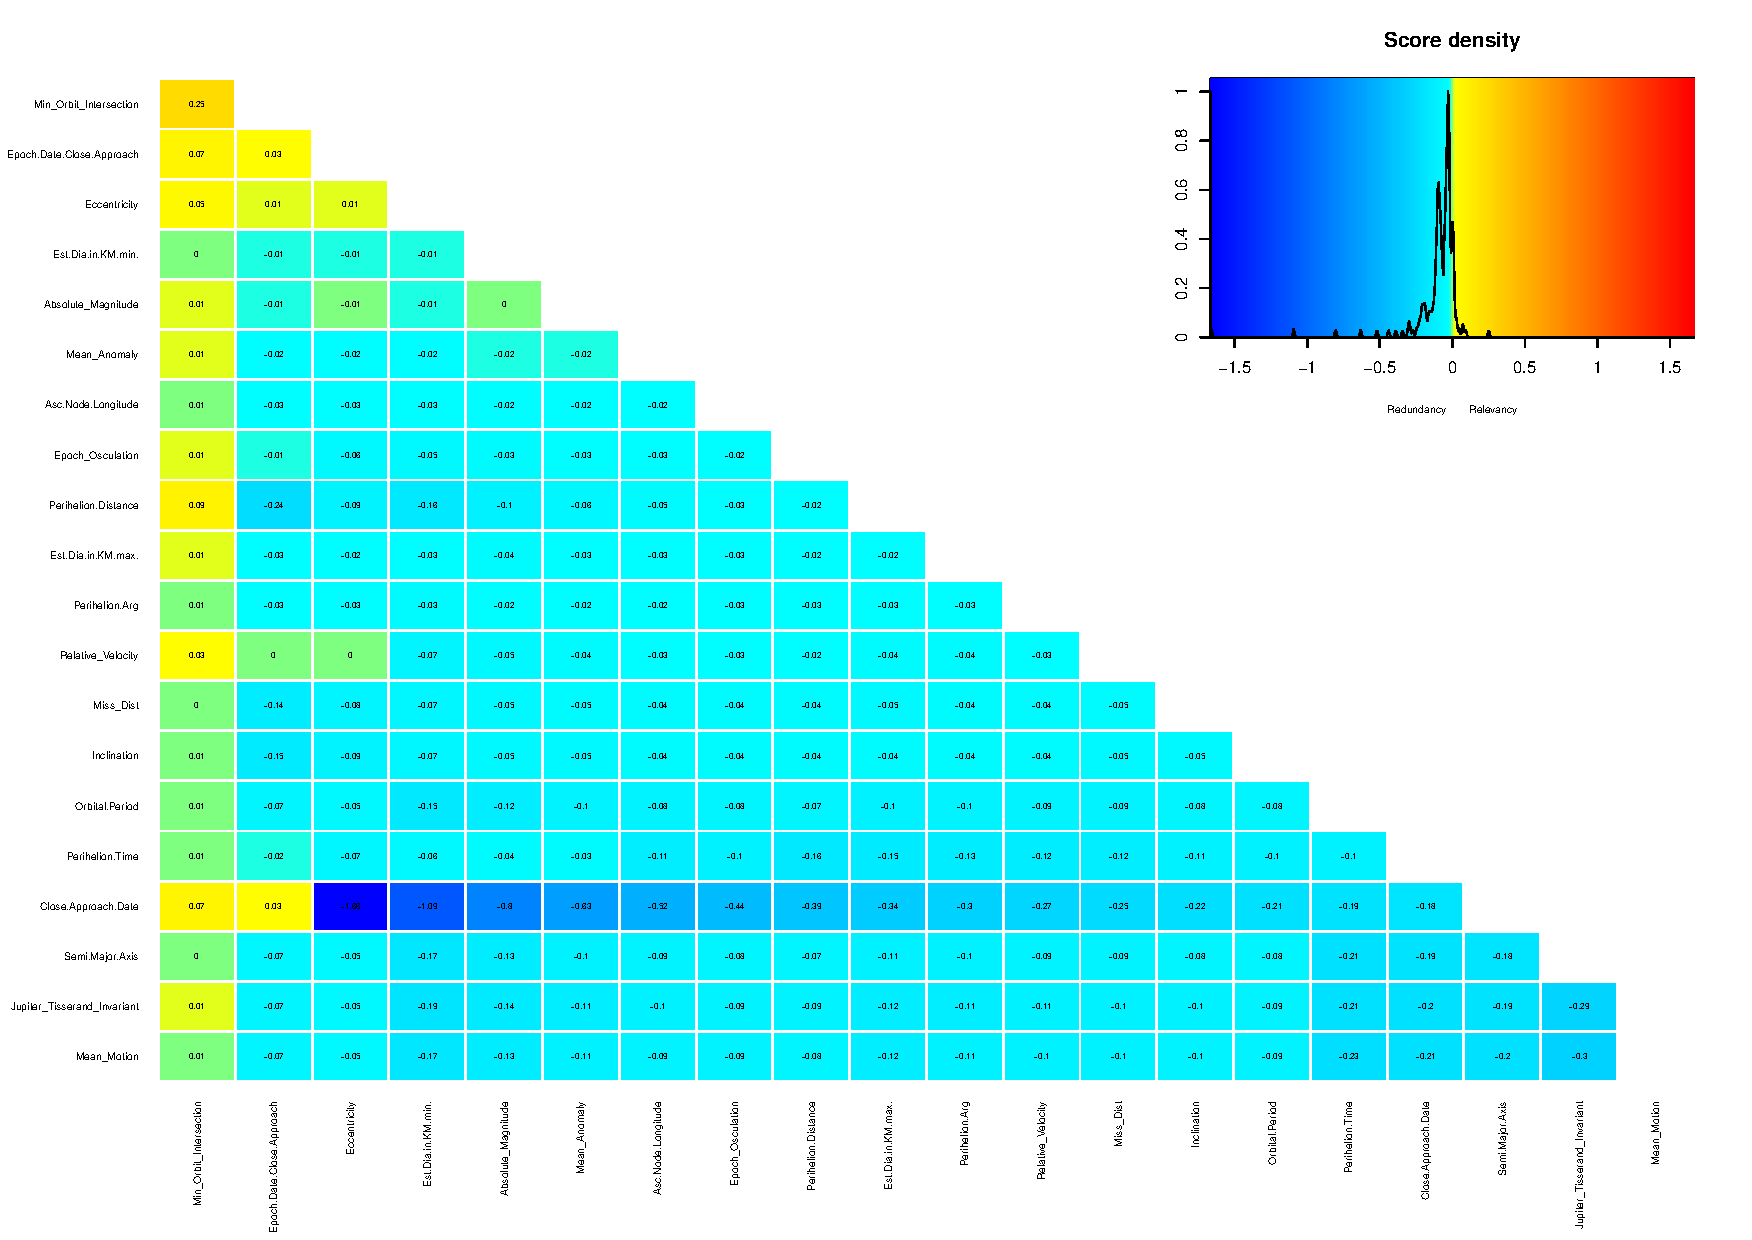
\includegraphics[width=1.75\textheight]{Figures/Mutual_information.pdf}
\caption{Mutual information as obtained with the varrank package \cite{kratzer2018varrank}}
\label{Mutual_information}
\end{center}
\end{figure}
\end{landscape}

\pagebreak

\section{Probabilistic models}

We started the analysis with the graphical models by inspecting the relations between continuous variables in the dataset: thus in this first step the binary variable \textit{Hazardous} was excluded. For this purpose, among the different methods available, we considered the \textit{Graphical least absolute shrinkage and selection operator} GLASSO as implemented in the \textit{glasso} R package \cite{friedman2008sparse,glasso}. After different tests reported in Fig. \ref{GLASSO_convergence}, we considered as final result the graph obtained with the value of $\rho$ (the one that penalize further connections) equal to $0.3$. This is because, in this plot, we see that the conditional dependences/independences stated by the Celestial Mechanics are correctly reproduced: for instance we see that the diameter of the asteroids is independent from all features related to its motion. This is definitely meaningful since the mass of the asteroids is largely lower with respect to the mass of earth: thus there is no way by which the asteroid orbit can be modified by its mass as explained in Appendix A. Furthermore we see that the Close approach Date and the Epoch date are dependant each other but in no way from the other features: this is right since the date and epoch are set with an arbitrary scale. Also the Perihelion Epoch and Osculation Time are dependant, as expected, but there is no dependence with the orbit parameters. We see that the mean motion is conditionally independent with respect to relative velocity, but correctly this is dependent from perihelion distance.
\begin{figure}[ht]
  \begin{minipage}[b]{0.5\linewidth}
    \centering
    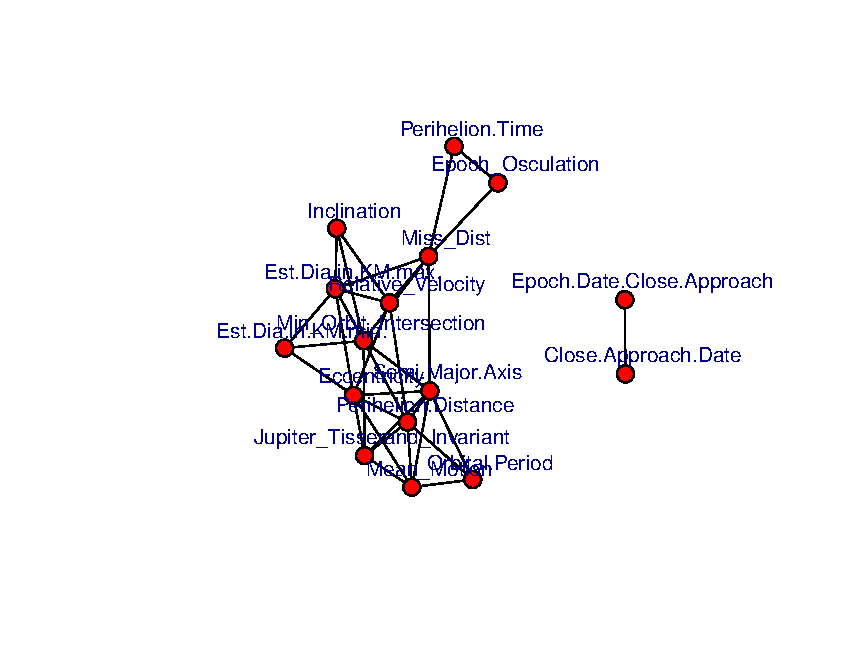
\includegraphics[width=.9\linewidth]{Figures/GLASSO_0.1.pdf}
    \subcaption{$\rho$=0.1}
    \vspace{4ex}
  \end{minipage} 
  \begin{minipage}[b]{0.5\linewidth}
    \centering
    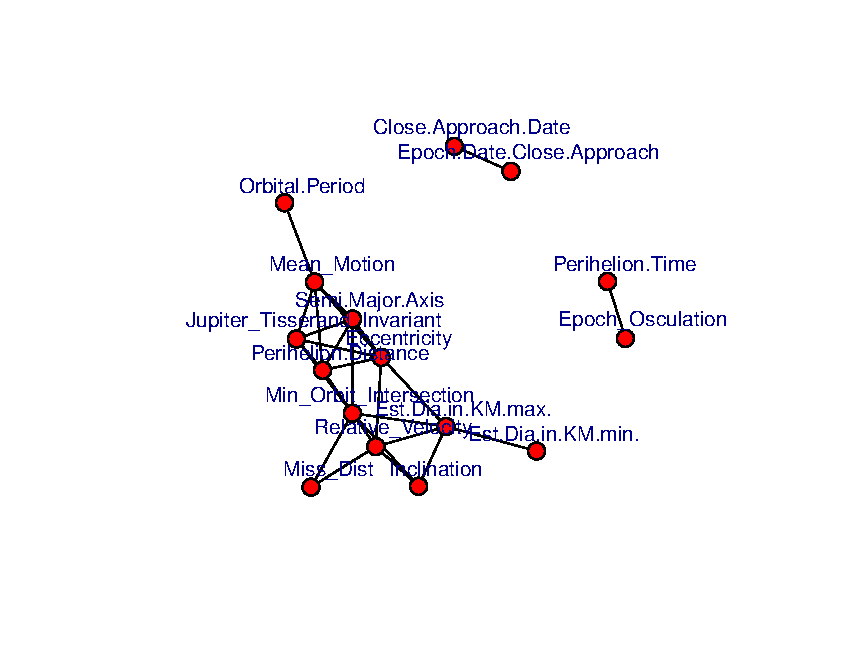
\includegraphics[width=.9\linewidth]{Figures/GLASSO_0.2.pdf}
    \subcaption{$\rho$=0.2}
    \vspace{4ex}
  \end{minipage} \\
  \begin{minipage}[b]{0.5\linewidth}
    \centering
    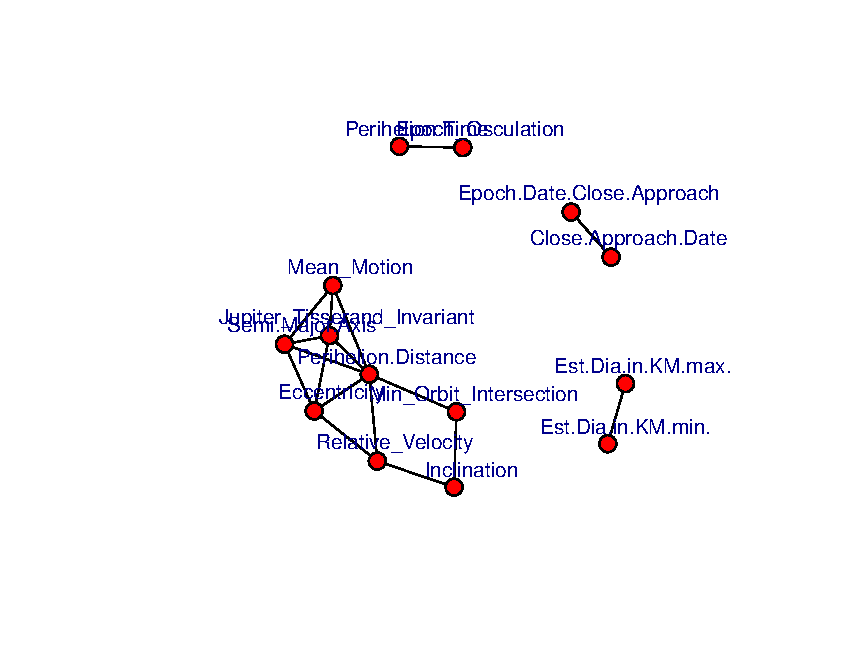
\includegraphics[width=.9\linewidth]{Figures/GLASSO_0.3.pdf}
    \subcaption{$\rho$=0.3}
    \vspace{4ex}
  \end{minipage}%%
    \begin{minipage}[b]{0.5\linewidth}
    \centering
    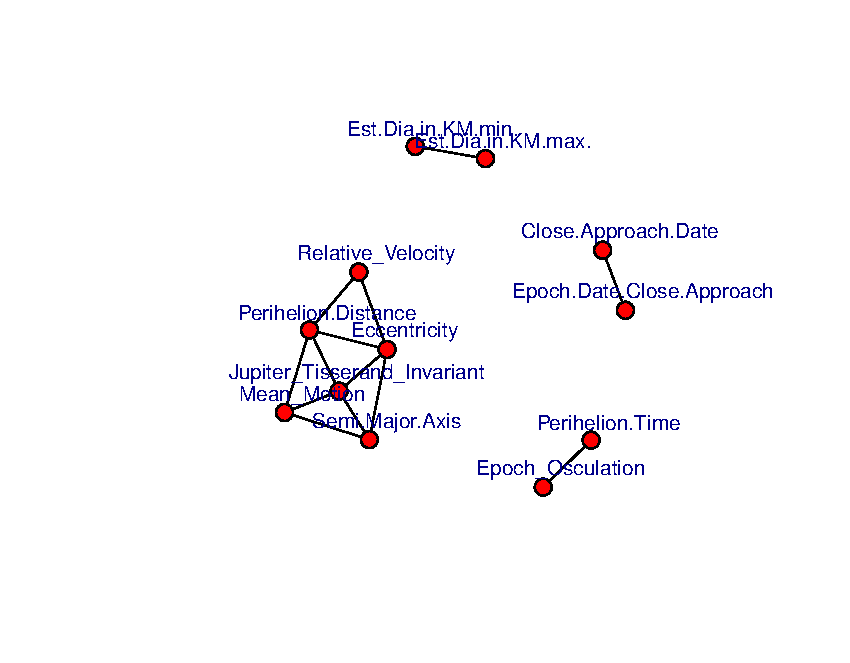
\includegraphics[width=.9\linewidth]{Figures/GLASSO_0.4.pdf}
    \subcaption{$\rho$=0.4}
    \vspace{4ex}
  \end{minipage}%%
\caption{GLASSO analysis, performed with the glasso package \cite{friedman2008sparse,glasso}, with different $\rho$ parameter (the one that penalize further connections) for the Asteroid dataset without the discrete variable Hazardous. The plots were obtained with the \textit{igraph} package for R \cite{igraph}}
\label{GLASSO_convergence}
\end{figure}
Lets now move on the mixed interaction model: first we considered its implementation in the mgm package \cite{mgm,haslbeck2015mgm}. We choose as $k$ parameter 2 and a cross validation (CV) with ten folds. The result is reported in Fig. \ref{mgm}. From this figure we see that the features that are conditionally dependant to the Hazardous features are: the absolute magnitude, the min orbit intersection, and the eccentricity.  All these connections are supported by the theory: the min orbit intersection is the main parameter for the hazardous value, the eccentricity on the other side can be tough as a parameter that describes how near the celestial body moves at the perihelion (indeed this parameter is correctly linked with the perihelion distance) and the Absolute Magnitude is also a meaningful parameter for the hazard evaluation since, if the asteroid is too small it will be destroyed by the earth atmosphere. It is worth mentioning that this parameter is correctly not connected with all quantities related to the orbital parameter except for the mean anomaly. Furthermore the parameters related to the diameters are also not connected with the orbital parameters. In addition we see also that the mean velocity is not directly related to the mean motion but there are the orbital parameters within them as expected. Thus it can be said that the model produced is almost consistent with the astronomic laws. On this basis, we can evaluate the performances of the model in term of confusion matrix, ROC curve and $\phi$ parameters (we used for this purpose the Caret R package \cite{kuhn2008building,caret}). The confusion matrix obtained is reported in Fig. \ref{mgm_confusion}: the ROC curve is given in Fig. \ref{ROC_mgm} and it corresponds to a $\phi=0.6$. We will comment these performances in a few when we will present the performances of other algorithms for the same dataset. Before this we would show the graphical models obtained with different implementation of mixed interaction model: we considered the function \textit{mmod()} of gRim package \cite{hojsgaard2012graphical} and the \textit{minforest()} of gRapHD (which uses the minForest method) \cite{de2009high}. Both were obtained with a stepwise algorithm.  Their result are reported in Fig. \ref{mmod} and \ref{minforest}. We see that in these models the minimum diameter is linked with the hazordous feature, and this is correct, but what is without a physical meaning is that this quantity is also linked to the features connected with the orbital parameters. Indeed, while for the magnitude (as for mgm model) a weak relationship can be admitted since this depends also on the distance between the asteroids and the observer and from the orbit, a volume and thus a mass dependence is not acceptable. In principle one can set these link as forbidden in the algorithm (blacklist), but in the author view it is preferable a model were the result is obtained without boundaries, instead of a one obtained with a large number of boundaries. Thus since a correct model was obtained without the imposition a blacklist, the mgm, we simply reject the mmod and minforest ones in favour of the first one. As consequence this is the reason why we report the performances of mgm model only. 


\begin{figure}[h]
\begin{center}
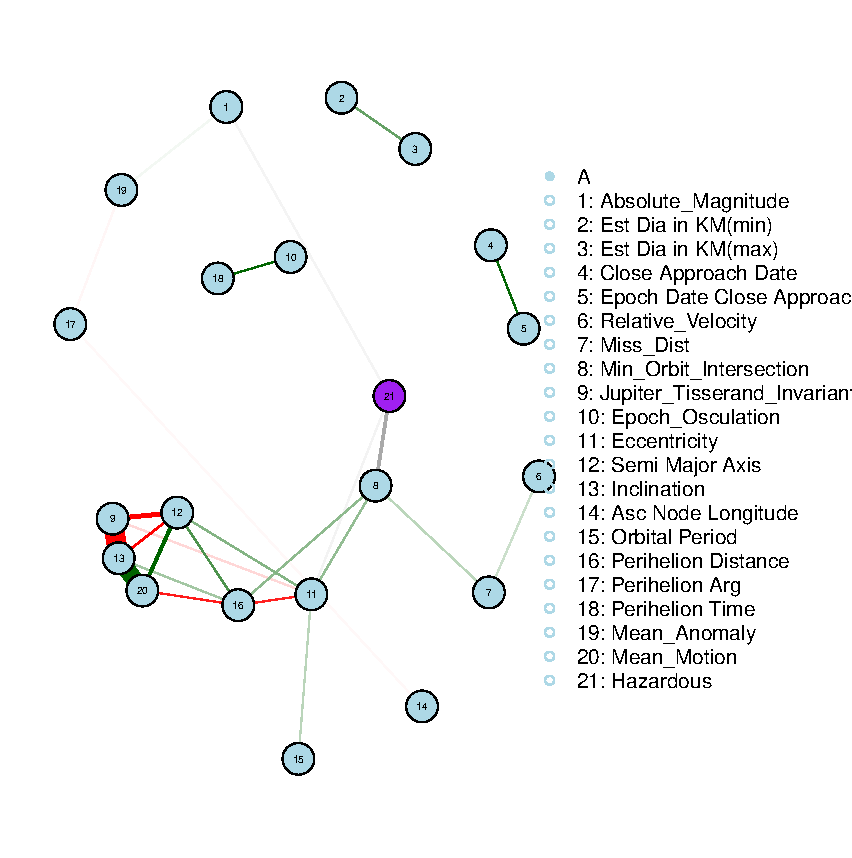
\includegraphics[width=1\textwidth]{Figures/mgm.pdf}
\caption{The graphical model obtained with the mixed interaction model as implemented in the mgm package \cite{mgm,haslbeck2015mgm}. The plot was obtained with the \cite{qgraph} package}
\label{mgm}
\end{center}
\end{figure}

\begin{figure}[h]
\begin{center}
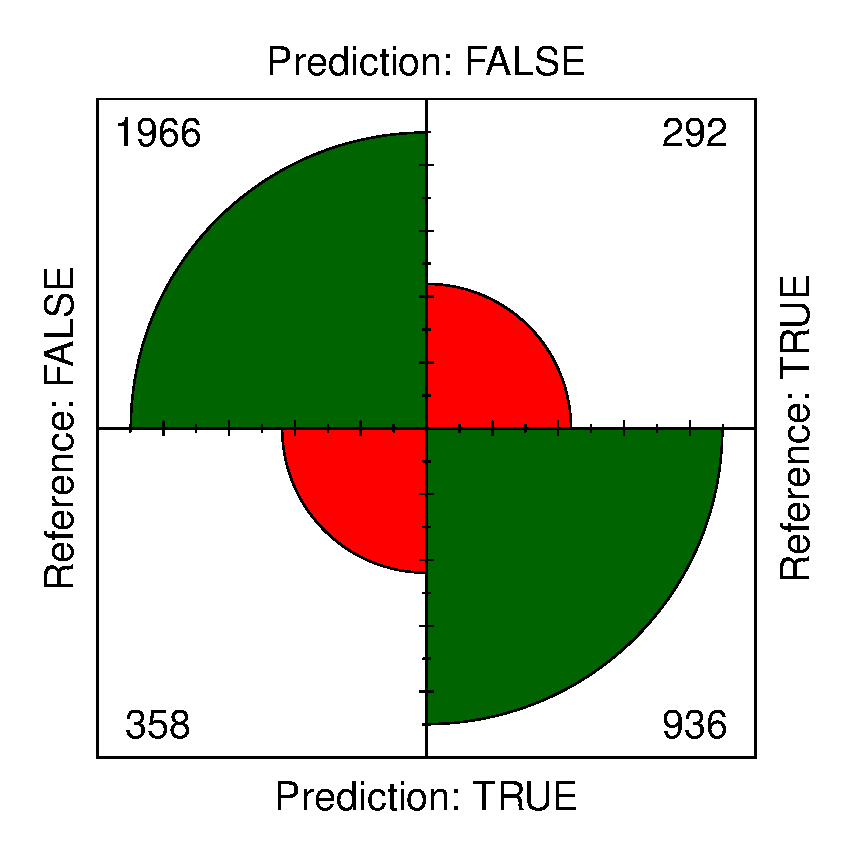
\includegraphics[width=1\textwidth]{Figures/mgm_confusion.pdf}
\caption{The confusion matrix of the graphical model reported in Fig. \ref{mgm} as obtained from the Caret package \cite{kuhn2008building,caret}} 
\label{mgm_confusion}
\end{center}
\end{figure}

\begin{figure}[h]
\begin{center}
\includegraphics[width=1\textwidth]{Figures/ROC_mgm.pdf}
\caption{The ROC curve as obtained from the ROCR package \cite{sing2005rocr} and ggplot2 \cite{ggplot2}. The corresponding $\phi$ value is $0.6$ } 
\label{ROC_mgm}
\end{center}
\end{figure}

\begin{landscape}
\begin{figure}
\begin{center}
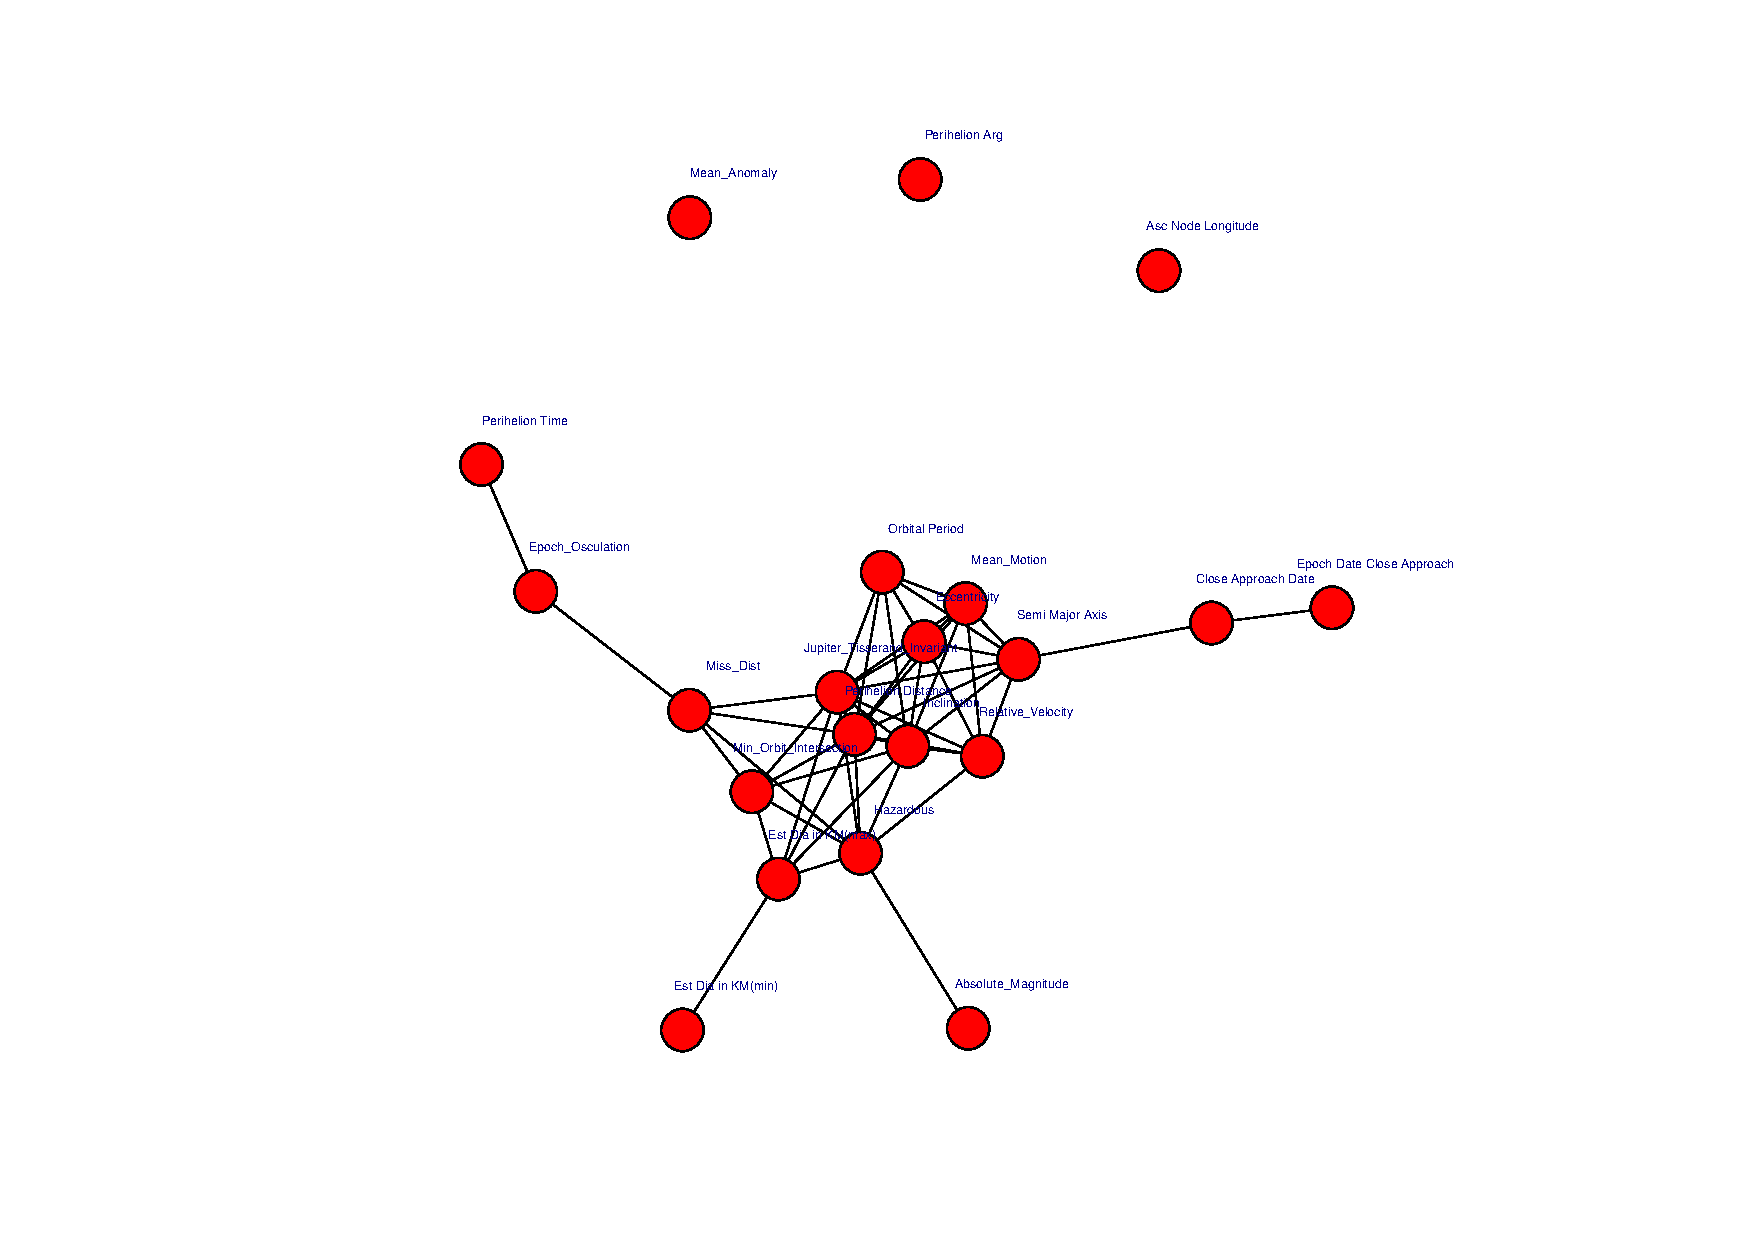
\includegraphics[width=1.5\textheight]{Figures/mmod.pdf}
\caption{The graphical mixed interaction model obtained with the grim package \cite{hojsgaard2012graphical}. The plot was obtained with the igraph package for R \cite{igraph} }
\label{mmod}
\end{center}
\end{figure}
\end{landscape}
\\
\begin{landscape}
\begin{figure}
\begin{center}
\includegraphics[width=1.5\textheight]{Figures/minforest.pdf}
\caption{The graphical mixed interaction model obtained with the gRapHD package \cite{de2009high} with a stepwise algorithm. The plot was obtained with the \cite{qgraph} package }
\label{minforest}
\end{center}
\end{figure}
\end{landscape}


\pagebreak

\section{Machine learning algorithms}

Given the mgm model as the one obtained with the probabilistic graphical methods, we would compare its performances with the ones obtained from the following machine learning algorithms: the random-forest (as implemented in the RandomForest package \cite{rfor}), the support vector machines (as implemented in the e1071 package \cite{dimitriadou2008misc}) , the quadratic discriminant analysis (as implemented in the MASS package \cite{MASS} and the logistic regression (as implented in stats package \cite{stats}). Their performances are reported in Fig. \ref{CF_ML} and \ref{ROC_mgm} as well in the Tab. \ref{phi_values}. From these comparison we can see that most of these algorithms, expect for the QDA outperform the graphical method mgm or have similar performances as for the logistic algorithm. Thus at this point one can ask what is the advantage of using a graphical method instead of a random forest or a SVM since its performances seems lower. The answer is the interpretability of the model provided: the random forest, at lest, can provide a variable rank importance as reported in Fig. \ref{RF_Importance} (note that apart from the Min Orbit intersection, there is a slight reshuffling in the feature importance with respect to the one established by the MI in fig \ref{Mutual_information}; however apart from this is a black-box as the SVM, the logistic regression and the QDA. Differently the probabilistic graph, providing the conditional independences, give to the user a interpretable model whose properties can be also compared, discussed and validated with the theory. Thus the model developed in this way allows a more scientific evaluation with respect to the black-box one. In the author view this characteristic definitely compensates the lack of predictive power with respect to the Random Forest or the SVM methods.


\begin{figure}[ht]
  \begin{minipage}[b]{0.5\linewidth}
    \centering
    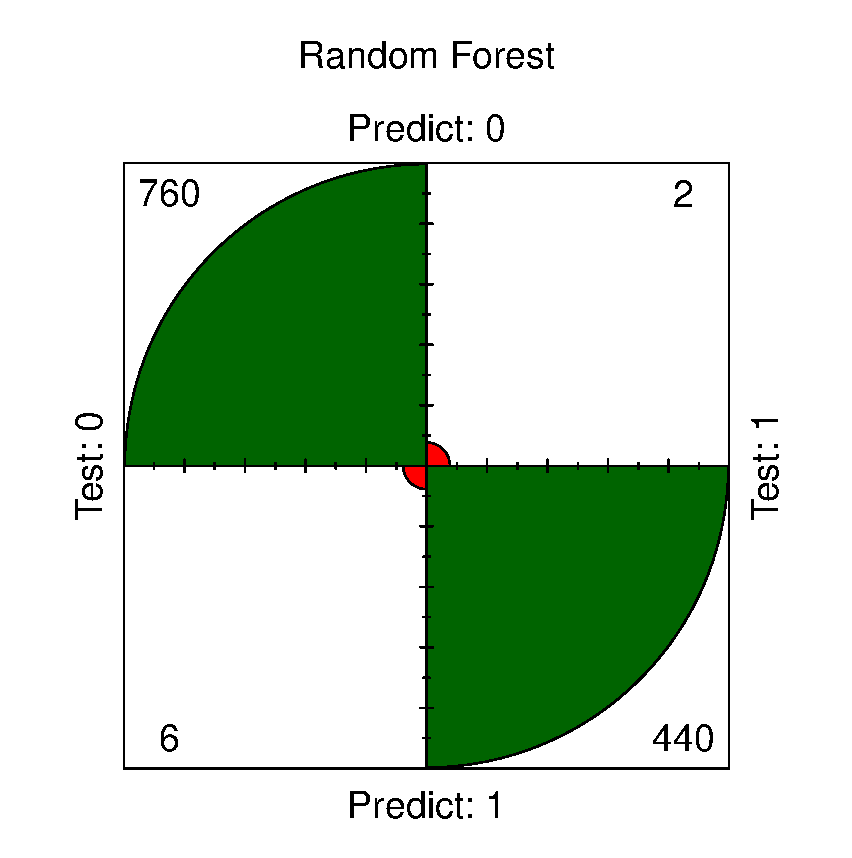
\includegraphics[width=.9\linewidth]{Figures/RF_confusion.pdf}
    \subcaption{Random Forest}
    \vspace{4ex}
  \end{minipage} 
  \begin{minipage}[b]{0.5\linewidth}
    \centering
    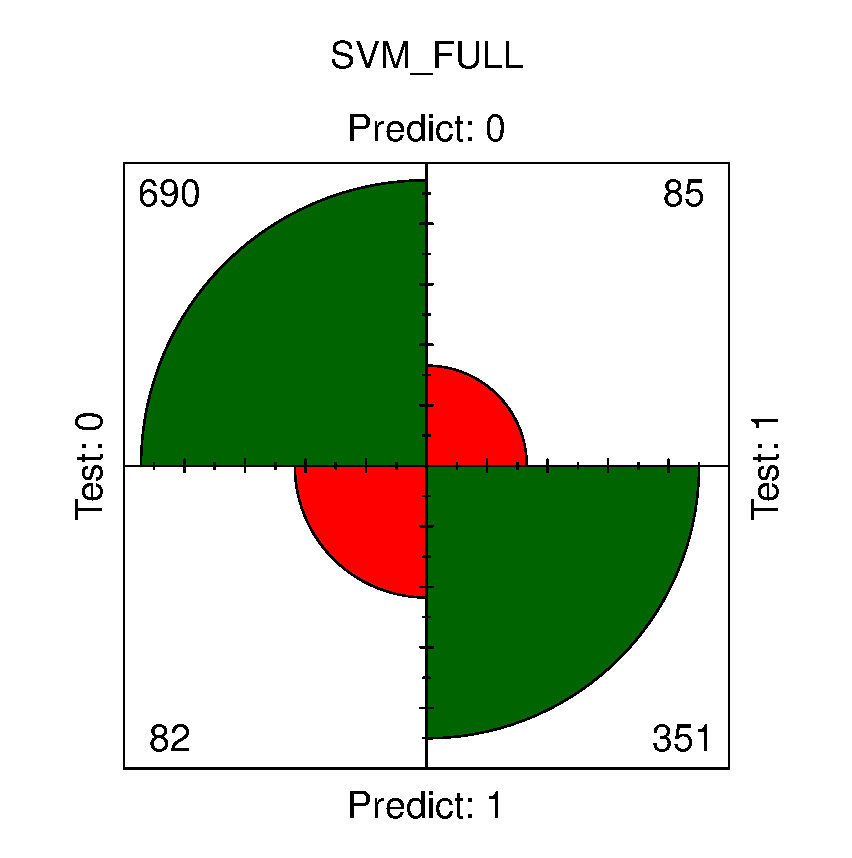
\includegraphics[width=.9\linewidth]{Figures/SVM_confusion.pdf}
    \subcaption{SVM}
    \vspace{4ex}
  \end{minipage} \\
  \begin{minipage}[b]{0.5\linewidth}
    \centering
    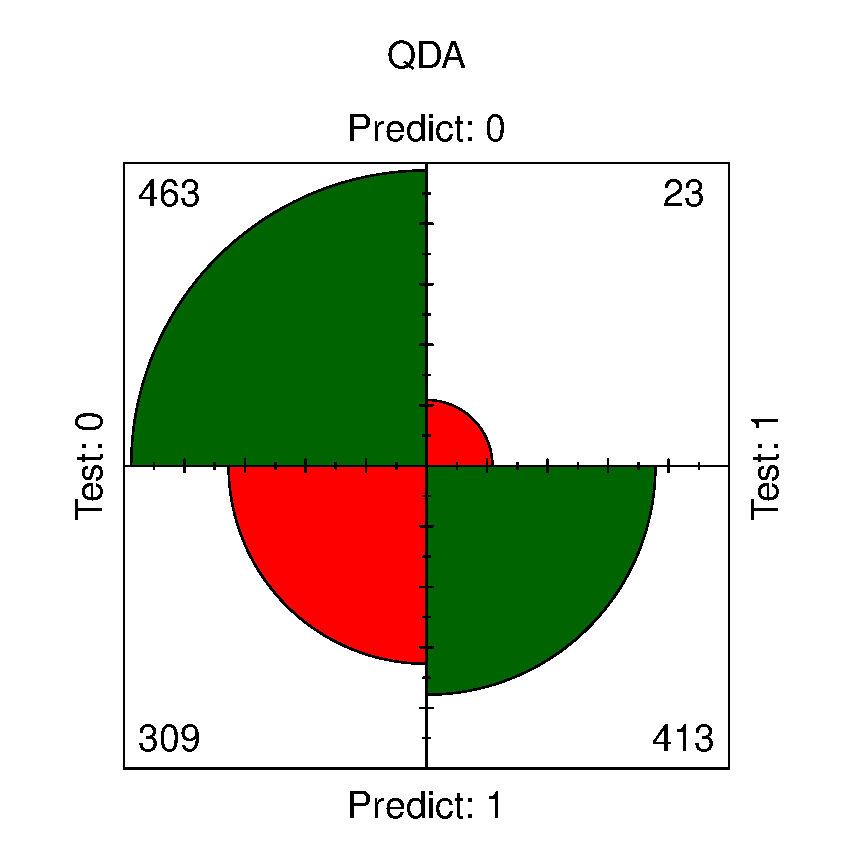
\includegraphics[width=.9\linewidth]{Figures/QDA_confusion.pdf}
    \subcaption{QDA}
    \vspace{4ex}
  \end{minipage}%%
    \begin{minipage}[b]{0.5\linewidth}
    \centering
    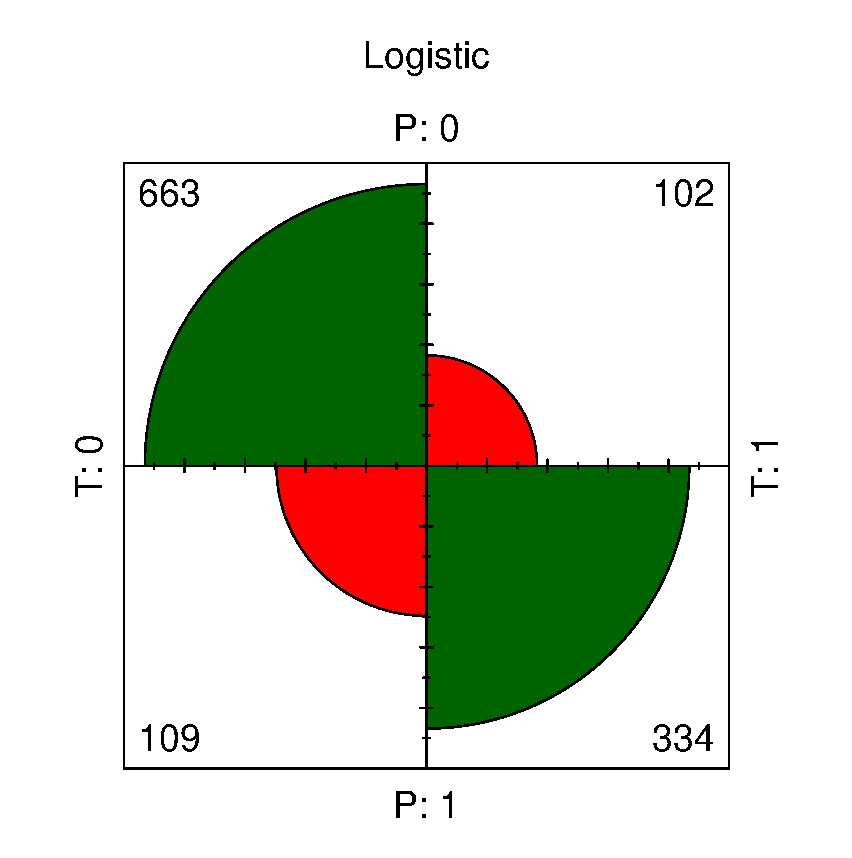
\includegraphics[width=.9\linewidth]{Figures/Logisic_confusion.pdf}
    \subcaption{Logistic}
    \vspace{4ex}
  \end{minipage}%%
\caption{Confusion matrices for a selected set of ML algorithms as obtained from the Caret package \cite{kuhn2008building,caret}}
\label{CF_ML}
  \end{figure}
  
  
  \begin{figure}[ht]
  \begin{minipage}[b]{0.5\linewidth}
    \centering
    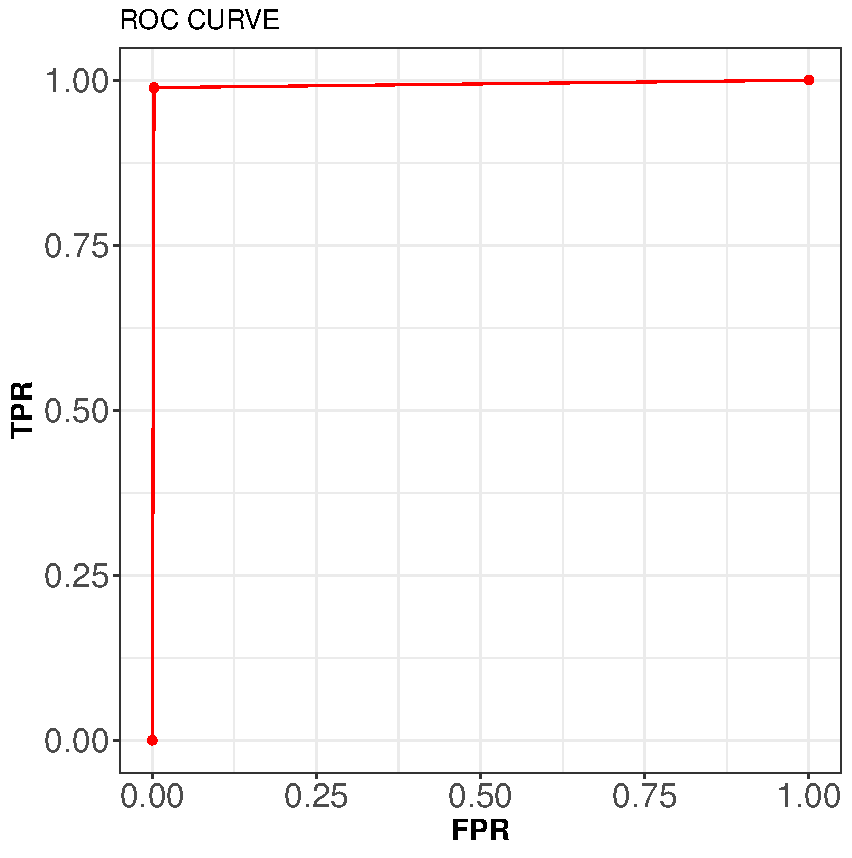
\includegraphics[width=.9\linewidth]{Figures/ROC_RF.pdf}
    \subcaption{Random Forest}
    \vspace{4ex}
  \end{minipage} 
  \begin{minipage}[b]{0.5\linewidth}
    \centering
    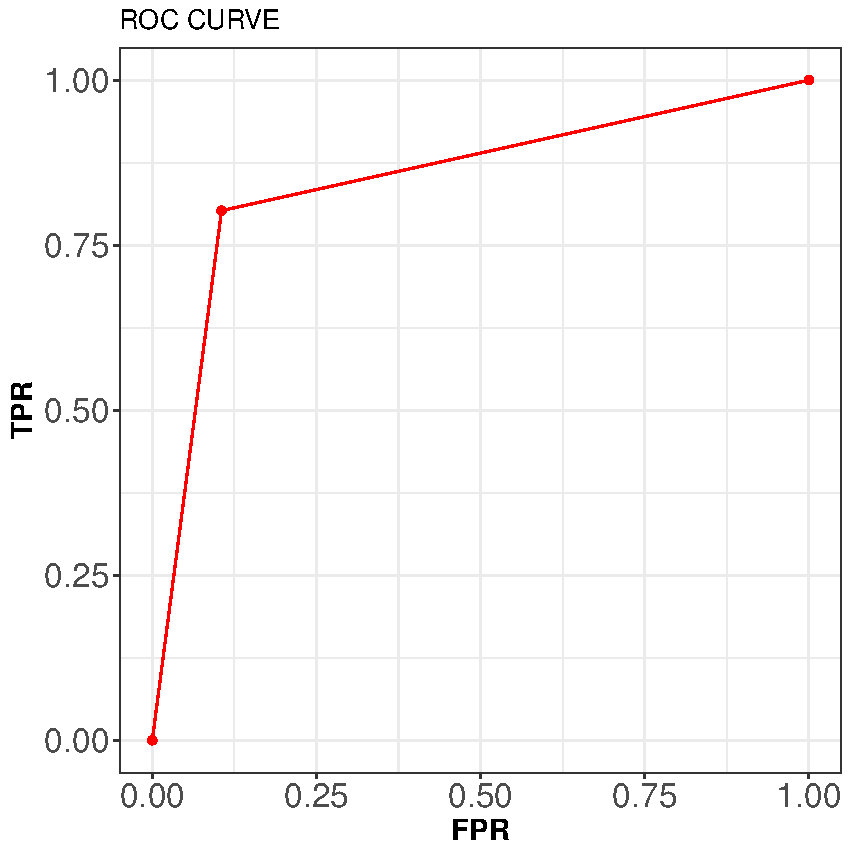
\includegraphics[width=.9\linewidth]{Figures/ROC_SVM.pdf}
    \subcaption{SVM}
    \vspace{4ex}
  \end{minipage} \\
  \begin{minipage}[b]{0.5\linewidth}
    \centering
    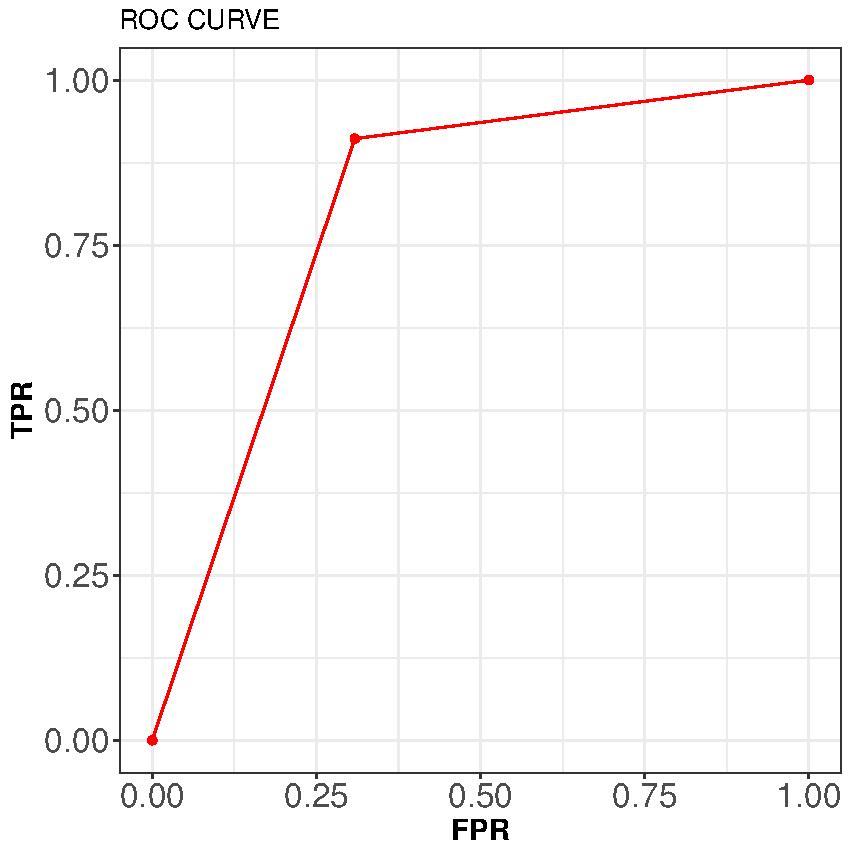
\includegraphics[width=.9\linewidth]{Figures/ROC_QDA.pdf}
    \subcaption{QDA}
    \vspace{4ex}
  \end{minipage}%%
    \begin{minipage}[b]{0.5\linewidth}
    \centering
    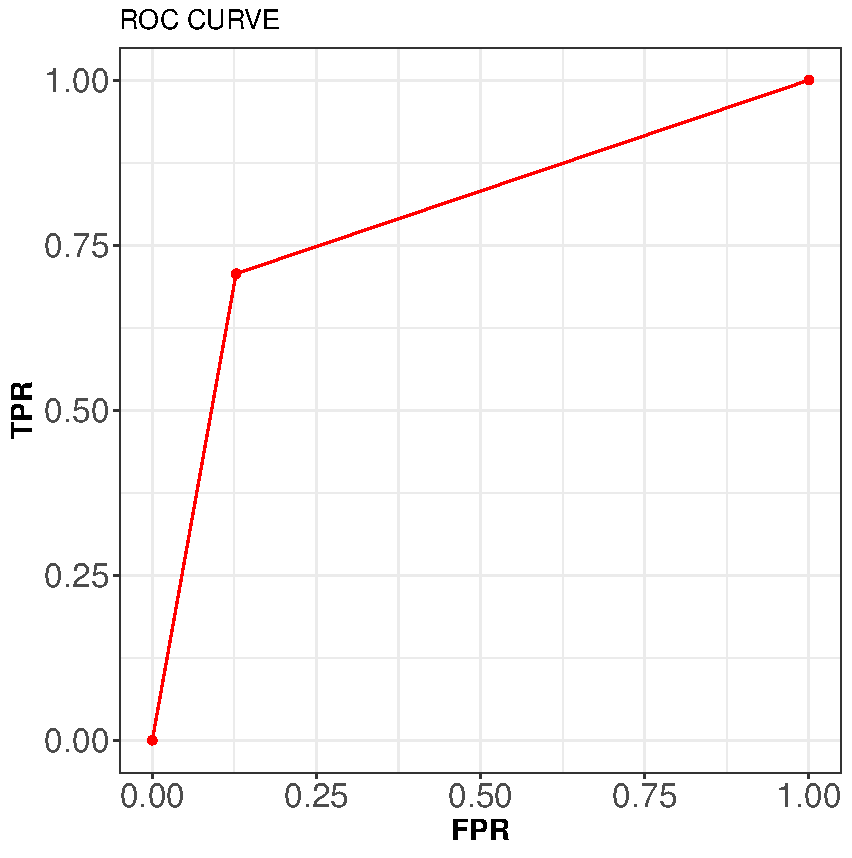
\includegraphics[width=.9\linewidth]{Figures/ROC_logistic.pdf}
    \subcaption{Logistic}
    \vspace{4ex}
  \end{minipage}%%
\caption{ROC curves for a selected set of ML algorithms. Plot obtained with caret and ggplot2 package \cite{kuhn2008building},ggplot2}}
\label{ROC_ML}
  \end{figure}



\begin{table}[]
\caption{$\phi$ factor for a selected set of ML algorithms as compared with the mgm}
\begin{center}
\begin{tabular}{c|c}
Algorithm & $\phi$ \\ \hline
RF        & 0.9876 \\ \hline
SVM       & 0.7111 \\ \hline
logistic  & 0.6173 \\ \hline
mgm       & 0.5997 \\ \hline
QDA       & 0.5562 
\end{tabular}
\end{center}
\label{phi_values}
\end{table}

\begin{figure}[h]
\begin{center}
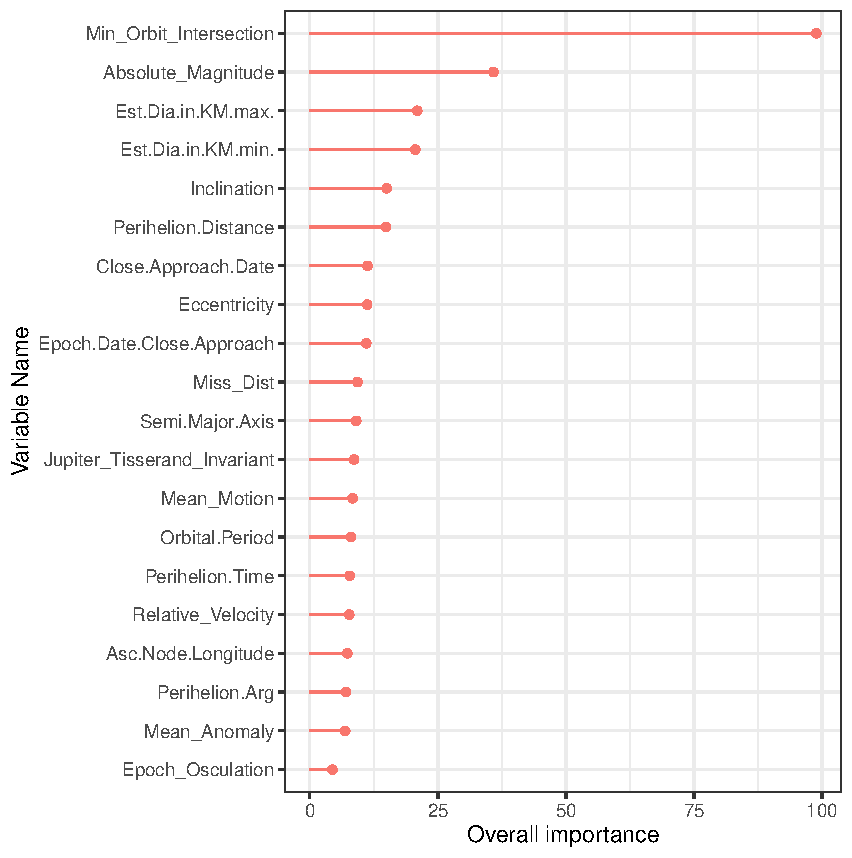
\includegraphics[width=1\textwidth]{Figures/RF_Importance.pdf}
\caption{Variable importance according to the random forest algorithm as implemented in \cite{rfor} package. Plot obtained with ggplot2 package \cite{ggplot2}}
\label{RF_Importance}
\end{center}
\end{figure}


\chapter{Conclusions}

The Glasso (with a penalizing parameter $\rho=0.3$) and the mgm algorithms provided graphical models that correctly capture the physical connections of the dataset feature. In particular for both models we saw that the no one of the orbital parameters are conditionally dependent with respect to the diameter of the asteroid, as stated by theory. Furthermore the mgm model is able to provide forecasts about the hazardousness of the asteroids with performances that are almost equal or better  than the logistic and QDA algorithms. On the other side the fact that its performances are lower with respect to the RF and SVM is definitely compensated by its interpretability. 


\chapter{Appendix A: Concepts of astronomy}

This Appendix is dedicated to review the basics concepts of astronomy that are needed to understand the features of the dataset and the theoretical framework in which these are involved. First the basic concepts of celestial mechanics will be recap following the Murray approach \cite{murray1999solar}: these will provide a description of the orbital parameters of the dataset. Then the concepts connected to the observation of the asteroids will be reviewed following the Burbine textboox \cite{burbine2016asteroids}. Finally, using the previous definition, the classification of the asteroids and in particular the definition of their hazardousness will be provided following the Center for Near-Earth Object Studies (CNEOS) statements \cite{nasa_classification}. 

\section{Celestial mechanics}

Lets start by considering two masses $m_{1}$ and $m_{2}$, which in the present case will be respectively the planet Earth and the asteroid. Their position will be given, respectively, by two vectors $\textbf{r}_{1}$ and $\textbf{r}_{2}$ considering the origin $O$ bounded in to an inertial space. Furthermore we can define also the relative position with the vector $\textbf{r}=\textbf{r}_{2}-\textbf{r}_{1}$. Since we suppose that the masses are not interacting with the electromagnetic force, these will be bounded only by the gravitational interaction which is given by the Newton law \cite{murray1999solar}:


\begin{equation}
\textbf{F}_{1}=\mathcal{G} \cdot \frac{m_{1}m_{2}}{r^{3}}\textbf{r}=m_{1} \ddot{\textbf{r}}_{1}
\end{equation}

\begin{equation}
\textbf{F}_{2}=-\mathcal{G} \cdot \frac{m_{1}m_{2}}{r^{3}}\textbf{r}=m_{1} \ddot{\textbf{r}}_{2}
\end{equation}

where $\mathcal{G}$ is universal gravitational constant, and the second equivalence is given by the second Newton law $\textbf{F}=m\cdot \textbf{a}$ in which $\textbf{a}$ is the acceleration calculated as the second derivative of the position vector \textbf{r}. Setting $\ddot{\textbf{r}}=\ddot{\textbf{r}}_{2}-\ddot{\textbf{r}}_{1}$ (thus we consider the motion of the second item with respect to the first one) and $\mu=\mathcal{G}(m_{1}+m_{2})$ the following differential equation will be obtained from the previous two ones \cite{murray1999solar}:

\begin{equation}
\dfrac{d^{2}\textbf{r}}{dt^{2}}+\mu\dfrac{\textbf{r}}{r^{3}}=0
\end{equation}


It can be seen that the $\textbf{r}$ and $\dot{\textbf{r}}$ lies always in the same plane: this is because the product vector $\textbf{r} \times \ddot{ \textbf{r}}=0$, thus if one integrates she will get that the product vector $\textbf{r} \times \textbf{r}=\textbf{h}$ where \textbf{h} is a constant vector. Furthermore the problem can be simplified by using polar coordinates  $\hat{\textbf{r}}$ and $\hat{\boldsymbol{\theta}}$. In this case speed and acceleration have the following form \cite{murray1999solar}:

\begin{equation}
\textbf{r}=r\hat{\textbf{r}}
\end{equation}

\begin{equation}
\dot{\textbf{r}}=\dot{r}\hat{\textbf{r}}+r\dot{\theta}\hat{\boldsymbol{\theta}}
\label{eq_dyn_nop}
\end{equation}

\begin{equation}
\ddot{\textbf{r}}=\left(\ddot{r}-r\dot{\theta}^{2}\right)\hat{\textbf{r}}+\left[\dfrac{1}{r}\frac{d}{dt}\left(r^{2}\dot{\theta}\right)\right]\hat{\boldsymbol{\theta}}
\end{equation}

Therefore the product vector between the speed and the position will have the following form \cite{murray1999solar}:

\begin{equation}
\textbf{h}=r^{2}\dot{\theta}\hat{\textbf{z}}
\end{equation}

where $\textbf{z}$ is a vector perpendicural to the plane, whose module is equal to \cite{murray1999solar}:

\begin{equation}
h=r^{2}\dot{\theta}
\end{equation}

If we consider the motion of the body $m_{2}$ in the time interval $\delta t$ we have that the area $\delta A$ illustrated in Fig \ref{Area_dynamics} will be \cite{murray1999solar}:

\begin{equation}
\delta A \approx \dfrac{1}{2} r(r+dr)\sin(\delta\theta) \approx  \dfrac{1}{2} r^{2}\delta\theta
\end{equation}

where the Taylor expansion at first order was used. Therfore  \cite{murray1999solar}:

\begin{equation}
\dfrac{dA}{dt}=\dfrac{1}{2}r^{2}\dfrac{d\theta}{dt}=\dfrac{1}{2}h
\end{equation}

but we know that $h$ is constant, therefore the first derivative, is constant. This is the $2^{th}$ Kepler law. Lets come back to the Eq. \ref{eq_dyn_nop}, if one recast it in polar coordinates, the following form will be obtained \cite{murray1999solar}:

\begin{equation}
\ddot{r}-r\dot{\theta}^{2}=-\frac{\mu}{r^{2}}
\end{equation}

This differential equation can be rewritten as an armonic oscillator with the  substitutions $u=\dfrac{1}{r}$ $h=r^{2}\dot{\theta}$ \cite{murray1999solar}:

\begin{equation}
\dot{r}=-\frac{1}{u}\dfrac{du}{d\theta}\dot{\theta}=-h\frac{du}{d\theta}
\end{equation}

\begin{equation}
\ddot{r}=-h\dfrac{d^{2}u}{d\theta^{2}}\dot{\theta}=-h^{2}u^{2}\frac{d^{2}u}{d\theta^{2}}
\end{equation}

\begin{equation}
\dfrac{d^{2}u}{d\theta^{2}}+u=\frac{\mu}{h^{2}}
\end{equation}

\begin{equation}
u=\frac{\mu}{h^{2}}\left[1+e\cos(\theta-\phi)\right]
\end{equation}

where the integration constants e and $\phi$ are respectively the amplitude and the phase. Therefore we have \cite{murray1999solar}:

\begin{equation}
r=\dfrac{p}{1+e\cos(\theta-\phi)}
\end{equation}

In this form we can recognize in $e$ the \textcolor{red}{eccentricity} and $p$ is the semilatus rectum \cite{murray1999solar}:

\begin{equation}
p=\frac{h^{2}}{\mu}
\end{equation}

Depening on the eccentricity we have four possible conics \cite{murray1999solar}:

\begin{itemize}
\item circle:  $e=0$ \quad $p=a$
\item ellipse: $0<e<1$ \quad $p=a$
\item parabola: $e=1$ \quad $p=2q$
\item hyperbola: $e>1$ \quad $p=a(e^{2}-1)$
\end{itemize}

in which $a$ is the semi-major axis of the conic. The shape of these orbits is reported in Fig. \ref{Elliptical_orbit}. All the asteroids considered here an eccentricity $0<e<1$, therefore they have an elliptical orbits in which the earth lies in to one of the two focal point. It is worth nothing that this is the first Kepler law.  Looking to Fig. \ref{Elliptical_orbit} we can define the point of minimum distance between $m_{1}$ and the orbiting body as the pericentre or \textcolor{red}{perihelion}, and the maximum distance as the apocentre or the aphelion. The \textcolor{red}{semi-major axis}, here denoted as $b$ on the other side is defined as the distance between the pericentre and the apocentre. Using the following identity \cite{murray1999solar}:

\begin{equation}
b^{2}=a^{2}(1-e^{2})
\end{equation}

we get \cite{murray1999solar}:

\begin{equation}
r=\frac{a(1-e^{2}}{1+e\cdot cos(\theta-\phi}
\label{eq-mot}
\end{equation}

Furthermore the third Kepler law, can be quickly obtained considering the area swept in one \textcolor{red}{orbital period} T (the time needed to complete a full round of the orbit) $A=\pi ab$. Since we know that this area is equal to $hT/2$ and $h^{2}=\mu a(1-e^{2})$ \cite{murray1999solar}:

\begin{equation}
T^{2}=\dfrac{4\pi^{2}}{\mu}a^{3}
\end{equation}

If we have two bodies, of masses $m$ and $m'$, that orbit around the Earth $m_{c}$, we can use the previous equation to obtain \cite{murray1999solar}:

\begin{equation}
\frac{m_{c}+m}{m_{c}+m'}=\left(\frac{a}{a'}\right)\left(\frac{T'}{T}\right)^{2}
\end{equation}

But since $m$,$m'<<m_{c}$ \cite{murray1999solar}:

\begin{equation}
(a/a')^{3}\approx(T/T')^{2}
\end{equation}

Therefore \cite{murray1999solar}:

\cite{murray1999solar}:

We see that the two orbital parameters $T'$ and $a'$ are independent with respect to orbiting mass. This statement can be extended to the other orbital parameters by considering the previous approximation $m$,$m'<<m_{c}$. This is why we expect that the mass/volume of the asteoroid can not be conditionally dependant to the orbital parameters. It is useful to define also the \textcolor{red}{mean motion} (feature that is also present in the asteroids dataset) as \cite{murray1999solar}:

\begin{equation}
n=\frac{2\pi}{T}
\end{equation}

Therefore \cite{murray1999solar}:

\begin{equation}
\mu=n^{2}a^{3}
\end{equation}

\begin{equation}
h=na^{2}\sqrt{1-e^{2}}=\sqrt{\mu a(1-e^{2})}
\label{eq_h}
\end{equation}

From which we can see that the angular velocity $\ddot{f}$ is function of the longitude. We are now going more in deep with this statement. Lets come back to the Eq. \ref{eq-mot}, this can be rewritten as \cite{murray1999solar}:

\begin{equation}
\dot{\textbf{r}}\cdot\ddot{\textbf{r}}+\mu\dfrac{\dot{r}}{r^{2}}=0
\end{equation}

whose integration gives \cite{murray1999solar}:

\begin{equation}
\frac{1}{2}v^{2}-\frac{\mu}{r}=C
\label{energy_cons}
\end{equation}

In which $v^{2}=\dot{\textbf{r}}\cdot\dot{\textbf{r}}$, and C the integration costant. This expression express the energy conservation: on the left side we have the \textit{vis-viva} term (basically the kinetic energy without the mass), on the right side the potential energy (rescaled with $\mu$). Lets come back to Eq. \ref{eq-mot}, and make the following substitution $f=\theta-\phi$, which is called the true anomaly. If we differentiate it we will obtain \cite{murray1999solar}:

\begin{equation}
\dot{r}=\frac{r\dot{f}e\sin f}{1+e\cos f}
\end{equation}


Remembering the the definition of $h=r^{2}\ddot{f}$, from Eq. \ref{eq_h} we have  \cite{murray1999solar}:

\begin{equation}
\dot{r}=\frac{na}{\sqrt{1-e^{2}}}e\sin f
\end{equation}

\begin{equation}
r\dot{f}=\frac{na}{\sqrt{1-e^{2}}}\left(1+e\cos f\right)
\end{equation}

Therefore \cite{murray1999solar}:


\begin{equation}
\begin{split}
v^{2}&=\dfrac{n^{2}a^{2}}{1-e^{2}}\left(1+2e\cos f +e^{2}\right)= \\
&=\dfrac{n^{2}a^{2}}{1-e^{2}}\left(\dfrac{2a(1-e^{2})}{r}-(1-e^{2})\right)
\end{split}
\end{equation}

\begin{equation}
v^{2}=\mu\left(\frac{2}{r}-\dfrac{1}{a}\right)
\end{equation}


From which we get that the \textcolor{red}{velocity} \footnote{In the dataset this quanitity is called relative velocity because the it the reference system is Earth} of the asteroid is maximum at the perihelion, and minimum at the aphelion. Their values that are equal respectively to \cite{murray1999solar}:

\begin{equation}
v_{perihelion}=na\sqrt{\dfrac{1+e}{1-e}}
\end{equation}

\begin{equation}
v_{aphelion}=na\sqrt{\dfrac{1-e}{1+e}}
\end{equation}

Another quantity that is contained in the asteroids dataset, and is useful to describe their orbits is the \textcolor{red}{mean anomaly}. This is defined as \cite{murray1999solar}:

\begin{equation}
M=n(t-\tau)
\end{equation}

where $\tau$, the time of pericentre passage, increases linearly with time at a costant rate equal to the mean motion. Furthermore is bounded by the following relations for the perihelion and aphelion \cite{murray1999solar}:

\begin{itemize}
\item $M=f=0$\quad$t=\tau$\quad Perihelion
\item $M=f=\pi$\quad$t=\tau+T/2$ \quad Aphelion
\end{itemize}

Such boundaries should be intended as periodic for multiple of the orbital period T. The geometrical interpretation of the angle associated to the mean anomaly is given in Fig. \ref{Mean_anomaly}. It can be proven (see \cite{murray1999solar}) that the value of this angle, which describe the position of the orbiting item, is given by the following expression, know as Kepler equation \cite{murray1999solar}:

\begin{equation}
M=E-e\sin E
\end{equation}

Finally as move on to space, other two angles are necessary for the description of an orbit: these are shown in Fig. \ref{Inclination} and are the \textcolor{red}{inclination} of the orbit (I) and the \textcolor{red}{longitude of the ascending node} $\Omega$. Given this quantities the Tisserard invariant can be calculated as \cite{murray1999solar}:

\begin{equation}
T_{P}=\frac{a_{p}}{a}+2\cos I\sqrt{\dfrac{a}{a_{p}}(1-e^{2})}
\end{equation}

If Jupiter is considered as perturbing body, we have the \textcolor{red}{Juptier Tisserard Invariant}. The underlying reason for this choice is to distinguish the Jupiter family comets ($2<T_{j}<3$) and the asteroids $T_{j}<2$. 


\section{Observation}

The luminosity of an asteroid can be quantified with the concepts of magnitude. It is worth pointing out that asteroids have no intrinsic luminosity, but instead reflects the radiation, usually not uniformly since they have no atmosphere, of stars or other celestial bodies with intrinsic luminosity. 
First of all, before defining the concept of magnitude is useful to provide the concept of radiation flux. In our case it can be though as the number of photons \footnote{One can think, at first approximation, photons as packet of energy associated to the emitted light. A more formal and complete description can be found in \cite{feynman2018feynman} } that moves across a sphere centred on the light source and with radius equal to the observer distance \cite{burbine2016asteroids}:

\begin{equation}
\Phi=\frac{L}{4\pi r^{2}}
\end{equation}

As one can note there is a dependence from $1/r^{2}$ which is given by the fact that the electromagnetic radiation, as for gravitational force, is spherically symmetric\footnote{A formal argument of this point can be found in \cite{zee2013einstein}}. On this basis, it is possible to define the relative magnitude as \cite{burbine2016asteroids}:

\begin{equation}
m=-2.5\log_{10}\Phi+C
\end{equation}

This definition is useful for the evaluation for the comparison between two light sources (e.g. two stars), since in this case we have \cite{burbine2016asteroids}:

\begin{equation}
m_{1}-m_{2}=-2.5\log_{10}\frac{\Phi_{1}}{\Phi_{2}}
\end{equation}

Finally the \textcolor{red}{Absolute magnitude} $M$ can be defined as the magnitude that the item will have if it is put at 1 AU\footnote{Astronomic Units, the distance between Earth and Sun: 1.49\cdot 10^{11} m} or 10 parsec \footnote{$3,08\cdot 10^{16}$ m. The physical meaning of this measure can be found in \cite{burbine2016asteroids}} from the observer. Therefore  \cite{burbine2016asteroids}:

\begin{equation}
M-m=-2.5\log_{10}\frac{\Phi\cdot d^{2} }{\Phi\cdot 10^{2}}
\end{equation}

where $d$ is the light source distance in parsec. Rearranging the terms we have \cite{burbine2016asteroids}:

\begin{equation}
M-m=-5\log_{10}\frac{ d^{2} }{10}+C
\end{equation}

\begin{equation}
M=m+5-5log_{10}d
\end{equation}



\section{Classification}

The solar system is composed not only by planets and the Sun, but also, as shown in Fig. \ref{Orbit_asteorids}, by a plethora of small bodies\footnote{Small with respect to the size of planets} whose orbit can be near to the Earth \cite{burbine2016asteroids}. In particular, if the orbit of these items is near less then 1.3 AU such items are called near-Earth object (NEO). Such items are of three type: comets, meteoroids and asteroids. The first one are icy bodies that moving near the sun melts and release gases giving coloured tails. Meteroids are small \footnote{With respect to asteroids} rocky/metallic items with a diameter less than 1 meter. Asteroids, on the other side, are items with a diameter larger than 1 m \cite{burbine2016asteroids}. The first two bodies are excluded from the present analysis. The near asteroids, which are mostly located on the sites reported in Fig. \ref{heic1715c}, are classified, as shown in Fig. \ref{neo_orbit_types}, according to their semi-major axis (a), perihelion distance (q), and aphelion distance (Q). Here we report the CNEOS definition \cite{nasa_classification}:

\begin{itemize}
\item \textbf{Atiras} $a < 1.0$ au $Q < 0.983$ au\quad \textit{NEAs whose orbits are contained entirely with the orbit of the Earth (named after asteroid 163693 Atira)}
\item \textbf{Atens} $a < 1.0$ au $Q > 0.983$ au \quad \textit{Earth-crossing NEAs with semi-major axes smaller than Earth's (named after asteroid 2062 Aten)}
\item \textbf{Apollos} $a>1.0$ au $q<1.017$ au \quad  \textit{Earth-crossing NEAs with semi-major axes larger than Earth's (named after asteroid 1862 Apollo) }
\item \textbf{Amors} $a>1.0$ au $1.017<q<1.3$ au \textit{Earth-approaching NEAs with orbits exterior to Earth's but interior to Mars' (named after asteroid 1221 Amor)}
\end{itemize}

Beside this classification, there is the one which involve the hazardousness of an asteroid \cite{nasa_classification}:

\begin{itemize}
\item \textbf{Potentially Hazardous Asteroids}: MOID $\leq 0.05$ au $M \leq22.0$ \textit{NEAs whose Minimum Orbit Intersection Distance (MOID) with the Earth is 0.05 au or less and whose absolute magnitude (M) is 22.0 or brighter}
\end{itemize}

This is the formal definition by which the asteroids contained in the dataset here analysed are classified as hazardous or not. 

\begin{figure}[h]
\begin{center}
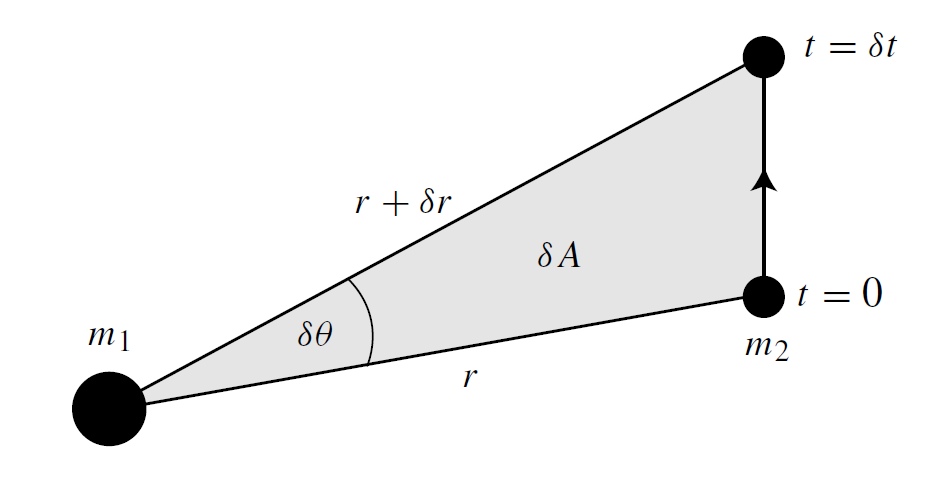
\includegraphics[width=1\textwidth]{Figures/Area_dynamics.png}
\caption{The portion of area $\delta A$ obtained when the position vector moves with an angle $\delta\theta$. Image taken from \cite{murray1999solar}}
\label{Area_dynamics}
\end{center}
\end{figure}

\begin{figure}[h]
\begin{center}
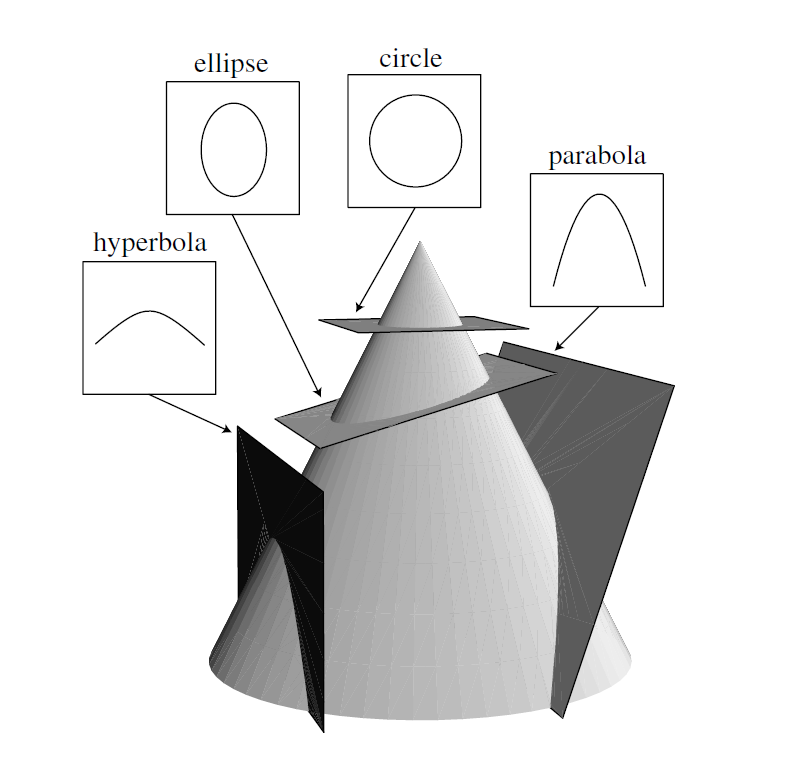
\includegraphics[width=1\textwidth]{Figures/Conics.png}
\caption{The four possible orbits as obtained from a sectionof a cone. Image taken from \cite{murray1999solar}}
\label{Conics}
\end{center}
\end{figure}

\begin{figure}[h]
\begin{center}
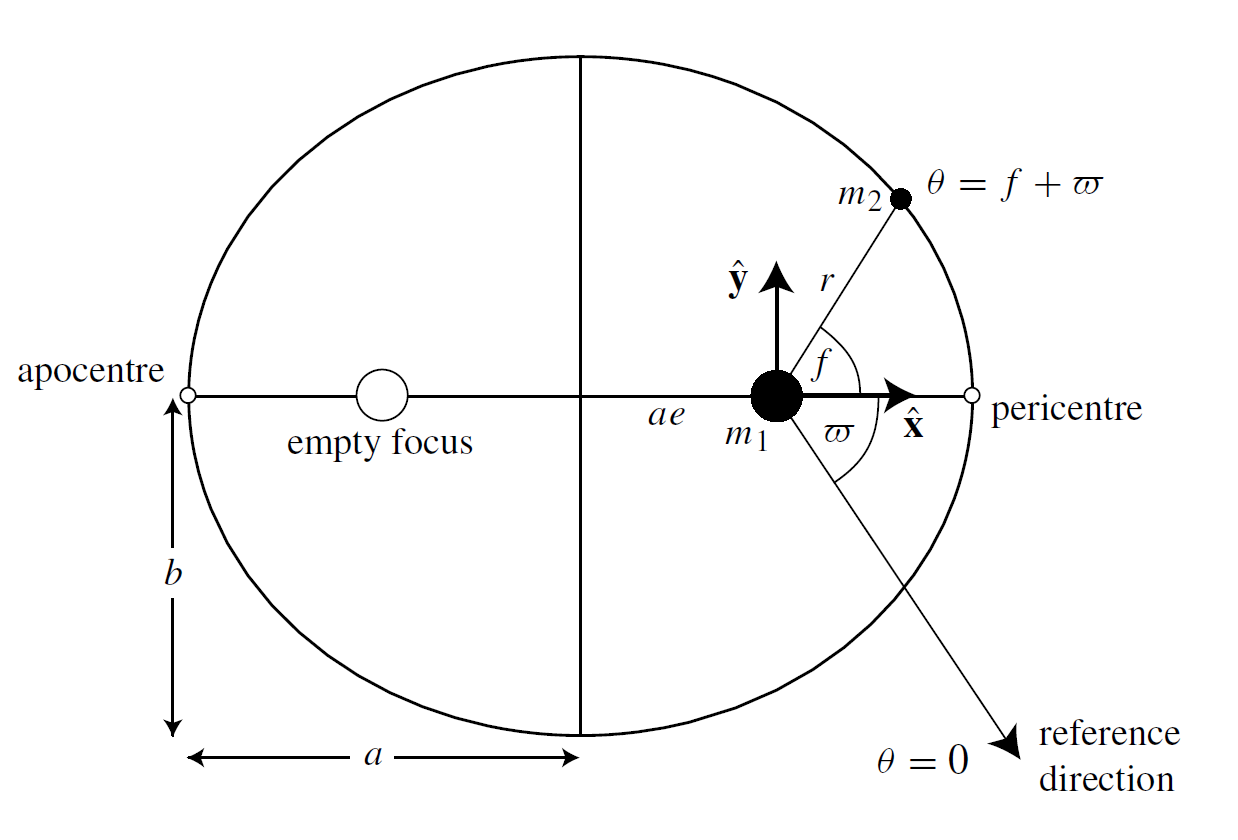
\includegraphics[width=1\textwidth]{Figures/Elliptical_orbit.png}
\caption{Main features of an elliptical orbit. Image taken from \cite{murray1999solar}}
\label{Elliptical_orbit}
\end{center}
\end{figure}

\begin{figure}[h]
\begin{center}
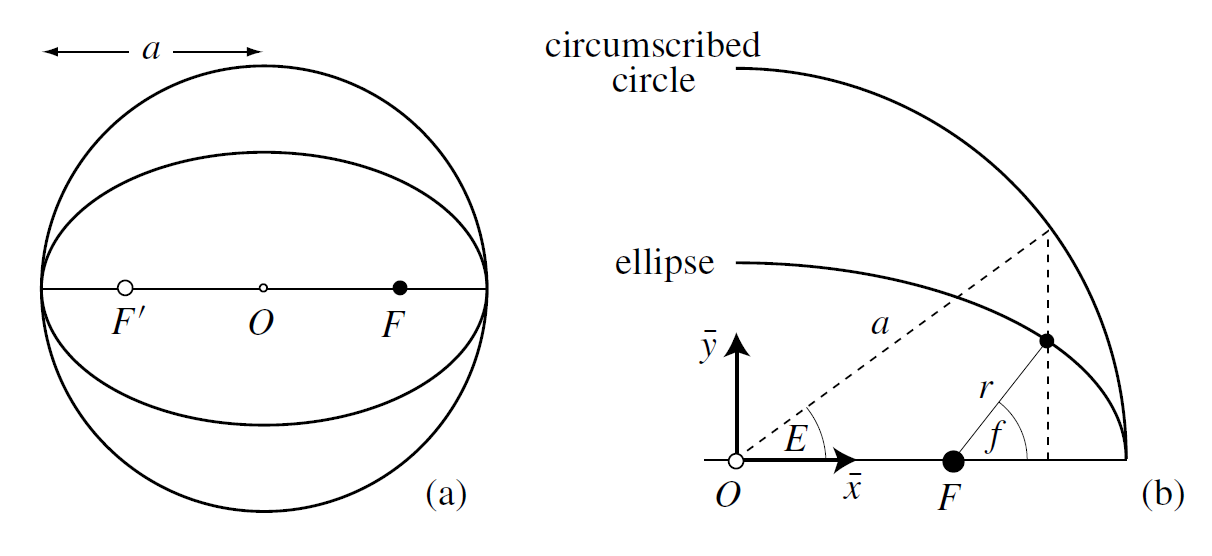
\includegraphics[width=1\textwidth]{Figures/Mean_anomaly.png}
\caption{The geometrical interpretation of mean anomaly: on the left panel a) is reported how the circumscribed circle should be draw, while on the right panel b) it is shown how the angle associated with the mean anomaly should be interpreted and its relation with the true anomaly angle f. Image taken from \cite{murray1999solar}}
\label{Mean_anomaly}
\end{center}
\end{figure}

\begin{figure}[h]
\begin{center}
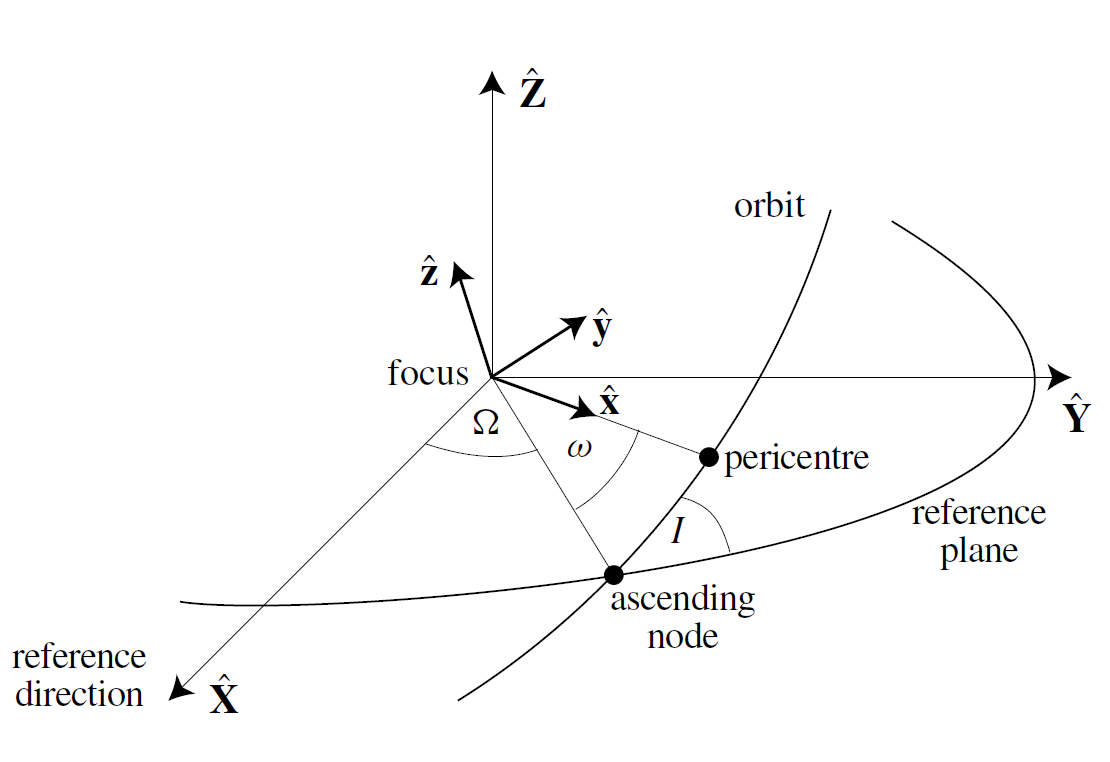
\includegraphics[width=1\textwidth]{Figures/Inclination.png}
\caption{The parameters that are necessary for the description of an orbit in three dimension. Image taken from \cite{murray1999solar}}
\label{Inclination}
\end{center}
\end{figure}


\begin{figure}[h]
\begin{center}
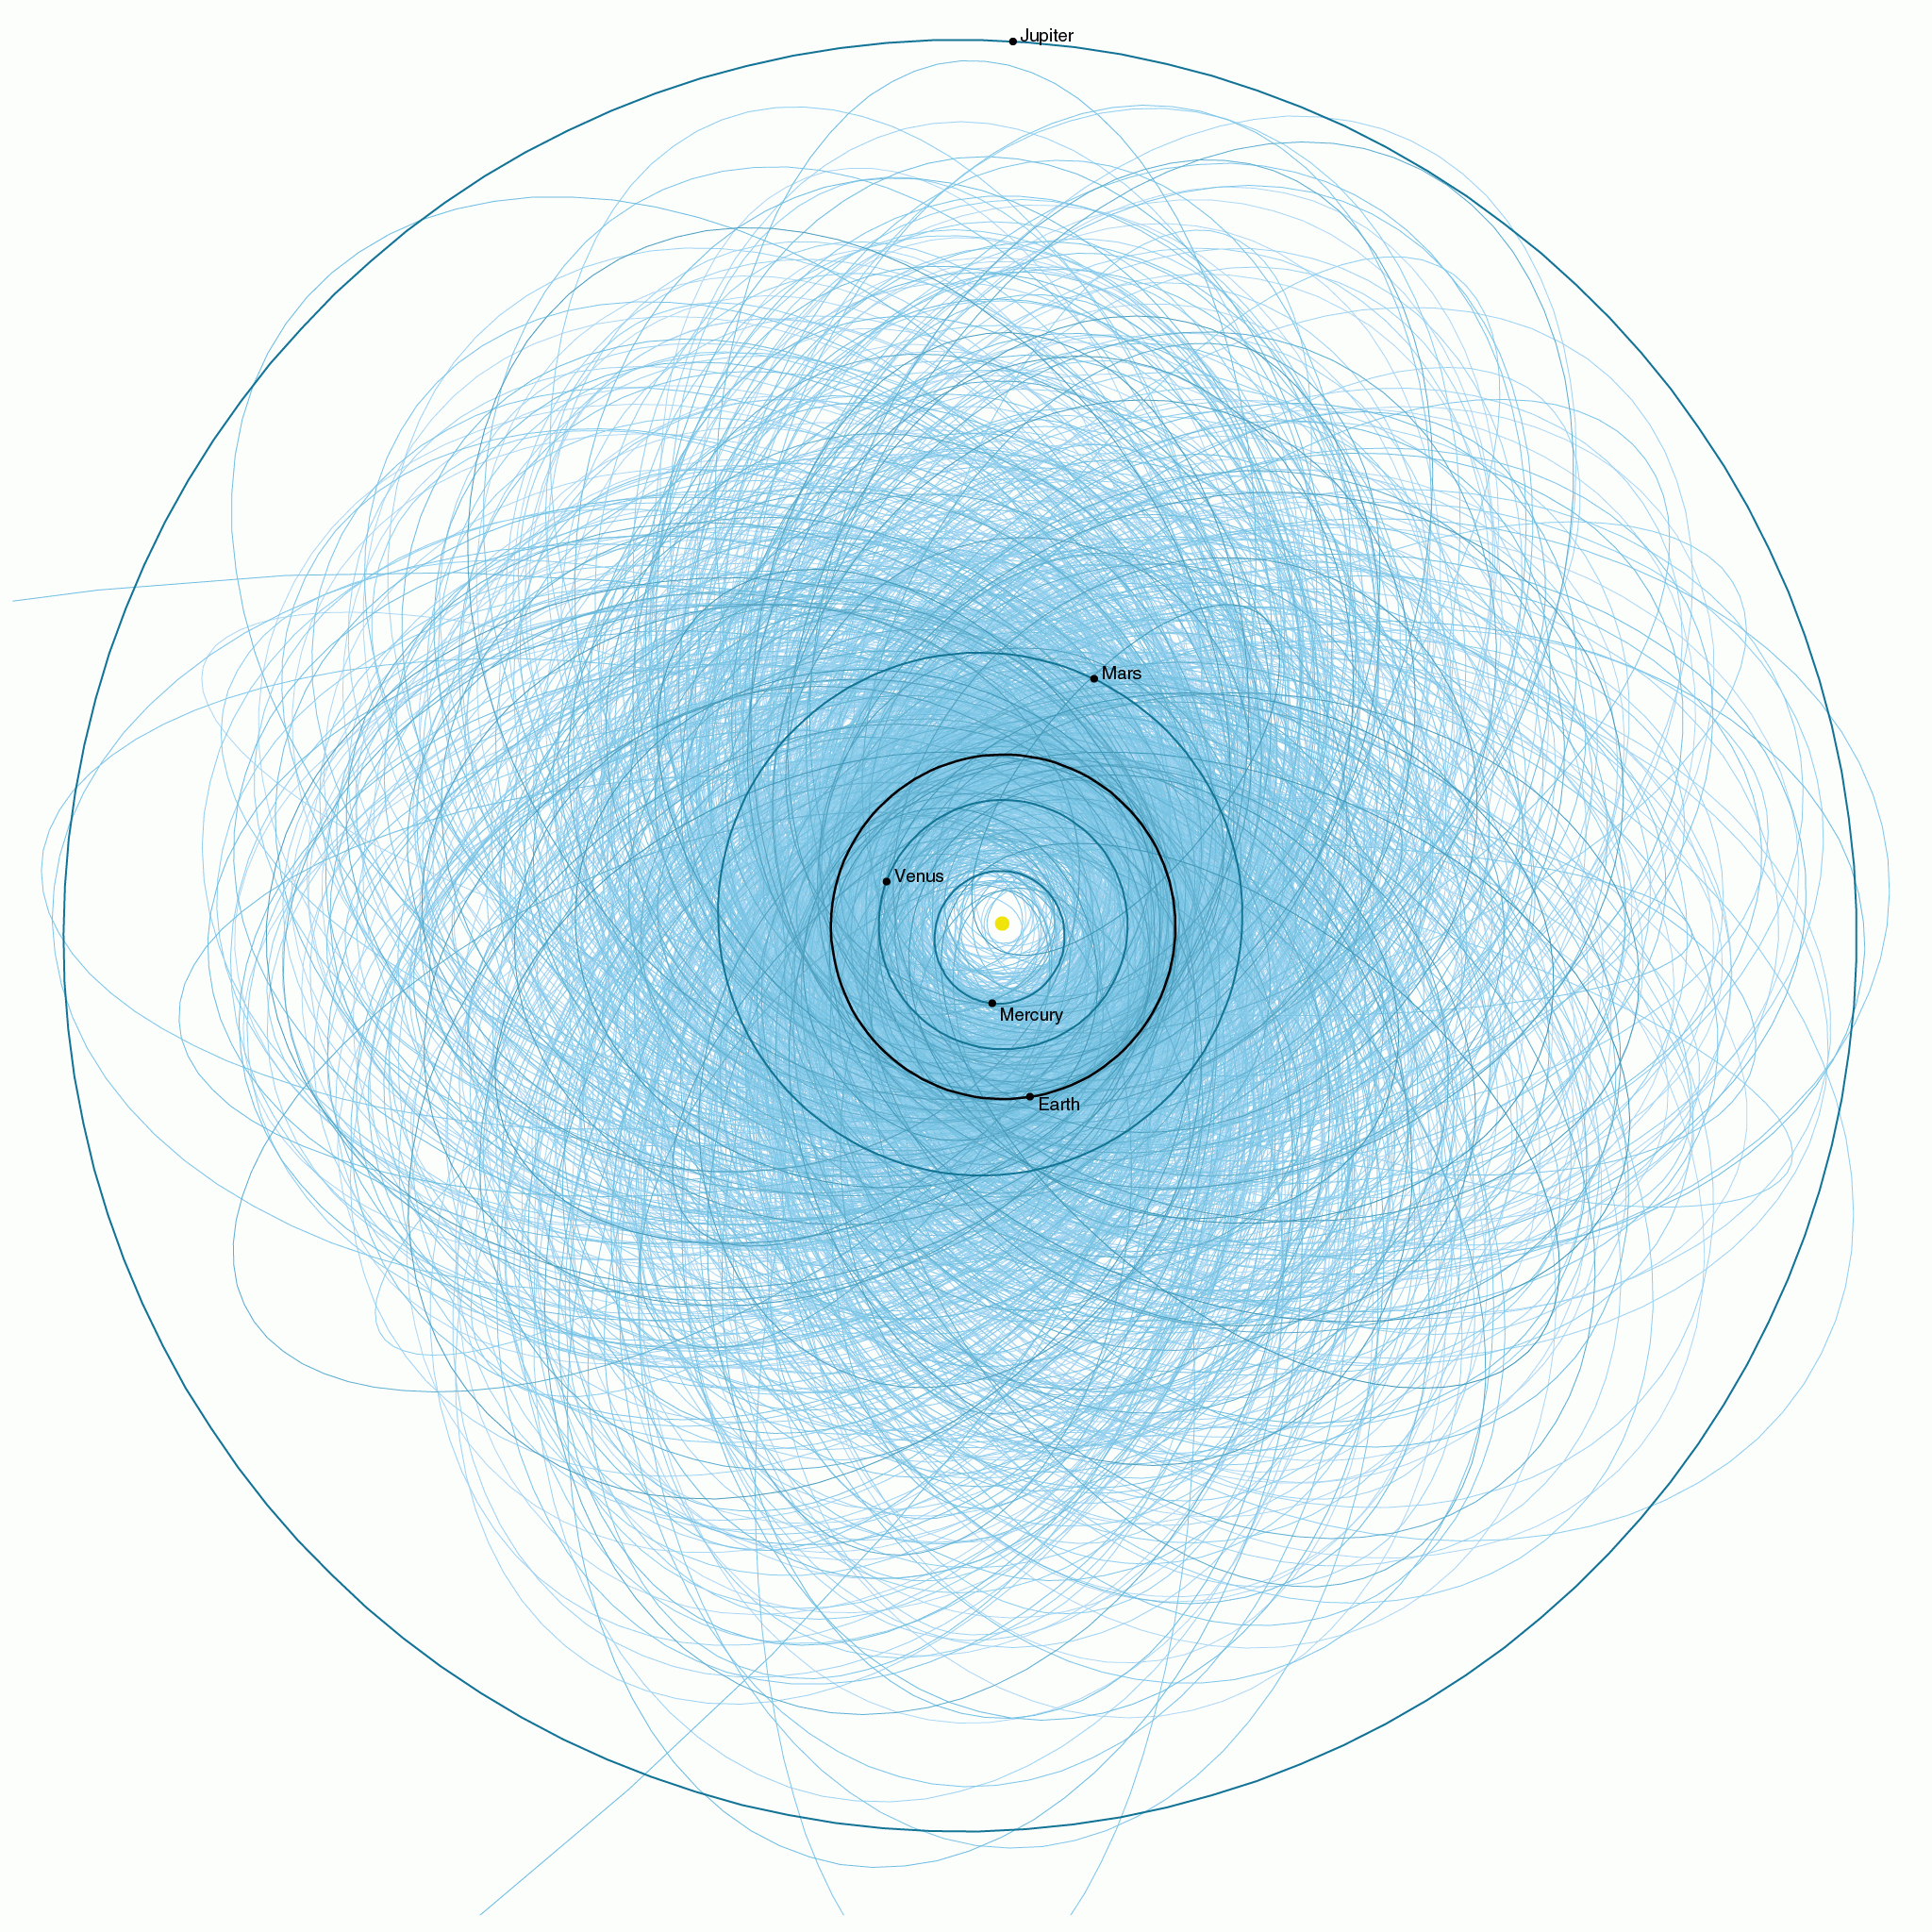
\includegraphics[width=1\textwidth]{Figures/Orbit_asteorids.png}
\caption{Orbits of potentially hazardous asteorids. Image taken from \cite{orbits-of-potentially-hazardous}}
\label{Orbit_asteorids}
\end{center}
\end{figure}

\begin{figure}[h]
\begin{center}
\includegraphics[width=1\textwidth]{Figures/heic1715c.jpg}
\caption{Location of the solar system asteroids belt. Image taken from \cite{esahubble}}
\label{heic1715c}
\end{center}
\end{figure}

\begin{figure}[h]
\begin{center}
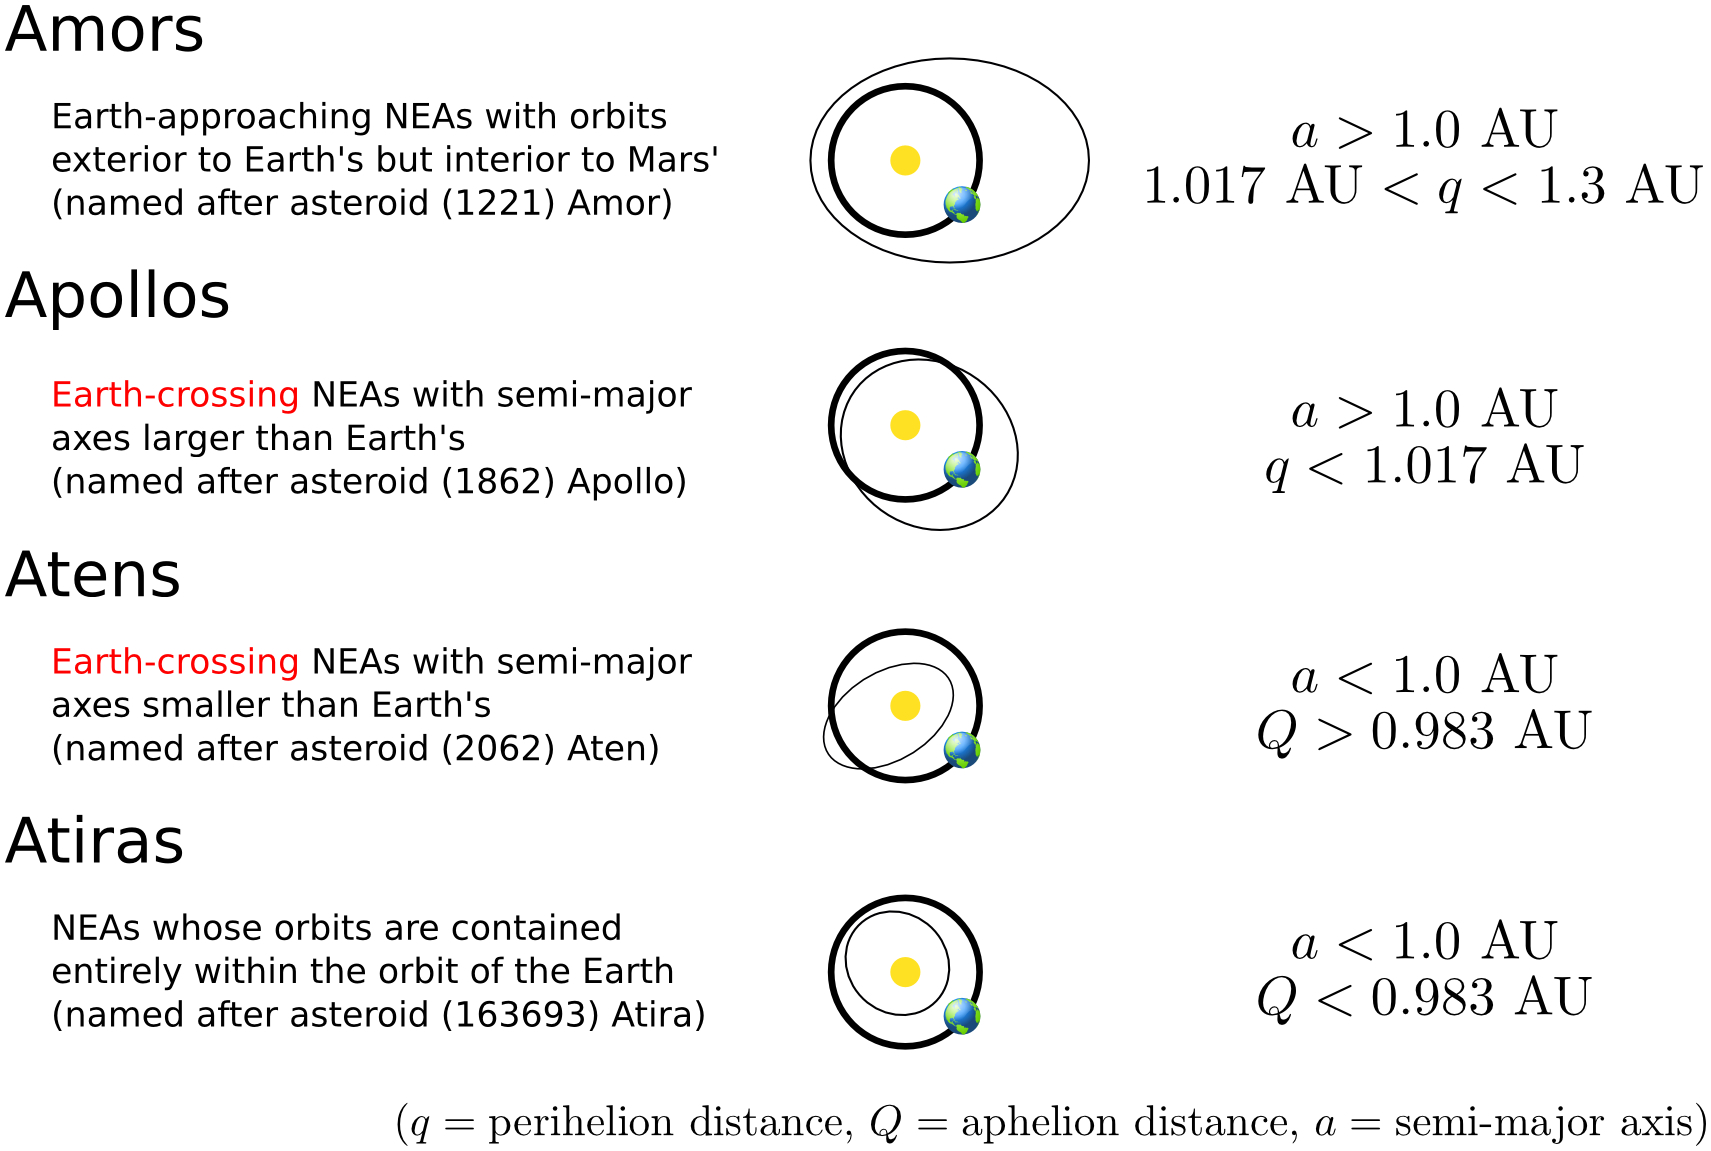
\includegraphics[width=1\textwidth]{Figures/neo_orbit_types.jpg}
\caption{NASA classification of NEO asteroids accompained by the legend for the parameters a,q and Q. Image taken from \cite{nasa_classification}}
\label{neo_orbit_types}
\end{center}
\end{figure}



\bibliographystyle{unsrt}

\bibliography{sample.bib} % The file containing the bibliography

\newpage



%----------------------------------------------------------------------------------------

\end{document}
